\chapter{Umsetzung}


\section{Motoransteuerung}

\subsection{Treiberbausteine}
Da die gewählten Akkus eine Spannung von 14,4V aufweisen, kann der orgiginal Motortreib erleider nicht verwendet werden.
Denn dieser benötig eine Spannung von 7,4V. Da der AVR Mikrokontroller mit 5V betrieben wird, wird ein Motorteiber benötig der
mit den 5V Pegeln arbeiten kann. In vielen Mikrocontroller Projekten und in unserem ersten Prototyp wird der L298 DUAL FULL-BRIDGE DRIVER
verwendet. Dieser ist leider auch bei der Benutzung beider Kanäle auf 4 Ampere begrenzt \cite{L298}, was beim Prototy zu einer Permanenten
überlastung des Treibers führt. Leider sind keine vollintegrierten Motortreiber mit der benötigten Belastbarkeit verfügbar.
Um die bentötigte Belastbarkeit zu erreichen wird der zur Ansteuerung benötigte Vierquadrantensteller aus diskreten Mosfets aufgebaut.

\subsubsection{Vierquadrantensteller}
Definition nach Wikipedia\cite{vierquadrantensteller}:\\
``Ein Vierquadrantensteller besteht aus einer elektronischen H-Brückenschaltung aus vier Halbleiterschaltern, meist aus Transistoren, 
welche eine Gleichspannung in eine Wechselspannung variabler Frequenz und variabler Pulsbreite umwandeln kann. Vierquadrantensteller 
in der Energietechnik können auch Wechselspannungen unterschiedlicher Frequenzen in beiden Richtungen ineinander umwandeln.''


\begin{figure}[H]
\centering
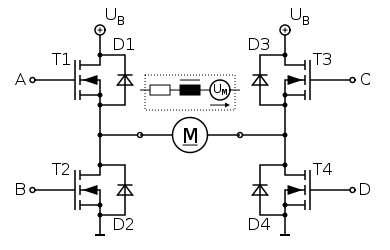
\includegraphics[width=.8\textwidth]{Vierquadrantensteller.png}\\
\caption{Vierquadrantensteller}%
\label{fig:Vierquadrantensteller}
\end{figure}


Auf Grund der hohen Belastbarkeit werden meißt Mosfets als Halbleiterschalter genutzt. Um die beiden oberen Mosfets (T1/T3) durchzuschalten
ist auf Grund des fehlenden Massepotentials eine Gatespannung oberhalb der Betriebsspannung nötig. Diese wird meist mittels Bootstrapping zur
Verfügung gestellt. Da das simultane Durchschalten der Übereinander liegenden Mosfets zu einem Kurzschluss führen würde, muss dies durch
eine Schutzschalung verhindert werden. Um all diese Funktionen zur verfügung zu stellen gibt es bereits fertige Mosfettreiber,
was das Schaltungsdesign enorm vereinfacht.

\subsection{Mosfettreiber}
\subsubsection{Verfügbarkeit}

Mosfettreiber gint es in vielenAusführungen, unter anderem als ``Single Channel High Side Driver``, ``Half Bridge Driver'', ``Full Bridge Driver''
und ``3 Phase Driver''. Da für den Verbauten DC-Motor eine Vollbrücke nötig ist, um den Motro in alle Richtungen zu betreiben, Werden an dieser Stelle
ausschließlich ``Full Bridge Driver'' untersucht.

Eine Tabelle auf Mikrocontroller.net\cite{FET_D_TABLE} zeigt eine Auswahl an verfügbaren Mosfettreibern. Dort sind zwei
``Full Bridge Driver'' aufgeführt, welche für dieses Projekt passend sind. Allerdings fällt die Entscheidung auf einen anderen Treiber,
dem Allegro A3941.
\subsubsection{Allegro A3941}
Der Allegro A3941 ist f+r Betriebsspannungen von 5,5V bis 50V geeignet und liegt damit in der Spezifikation des Projekts.
Des weiteren verfügt der Motor über eine integrierten 5V Regulator und kann somit ohne Spannungsregulator am Akku betrieben werden.
Über zwei Ausgänge der Treibers können diverse Fehler ausgelesen werden.


Der Treiber lässt sich in verscjiedennenModi betreiben:

\begin{figure}[H]
\centering
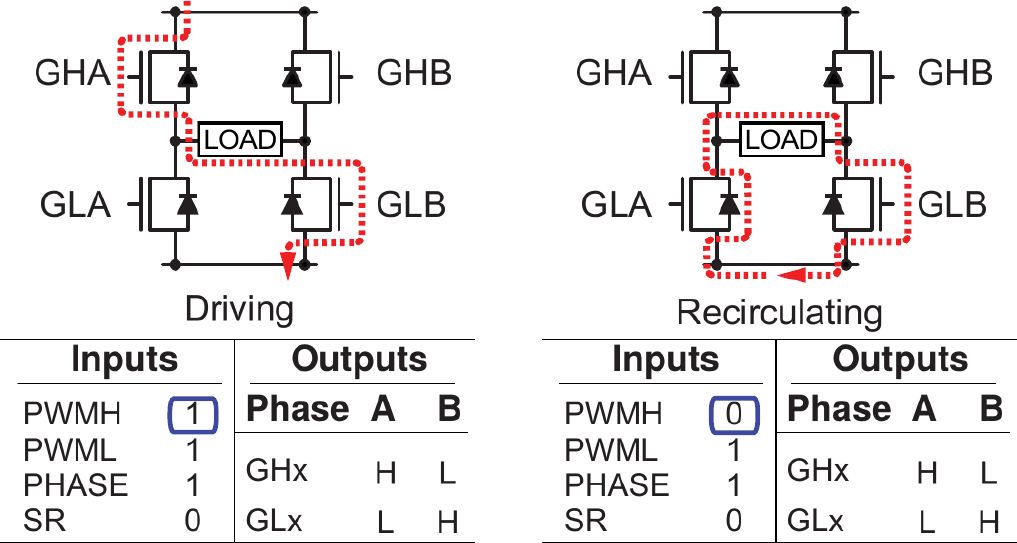
\includegraphics[width=.8\textwidth]{3941_1.png}\\
\caption{Slow decay, diode recirculation, high-side PWM}%
\label{fig:3941_1}
\end{figure}

Konfiguration: PWML=1, PHASE=1, SR=0 und PWM an PWMH (high-side PWM)\\
Bei aktivierten PWMH fließt der Strom durch den GHA-Mosfets über den Motor und
dann über den GLB-Mosfet. in diesem Modus wird der Motor angetrieben.
Wenn PWML deaktiviert ist zirkuliert der vom Motor induziert Strom durch GLB und durch
die interne Diode von GLA, der Motor wird dadurch gebremst.


\begin{figure}[H]
\centering
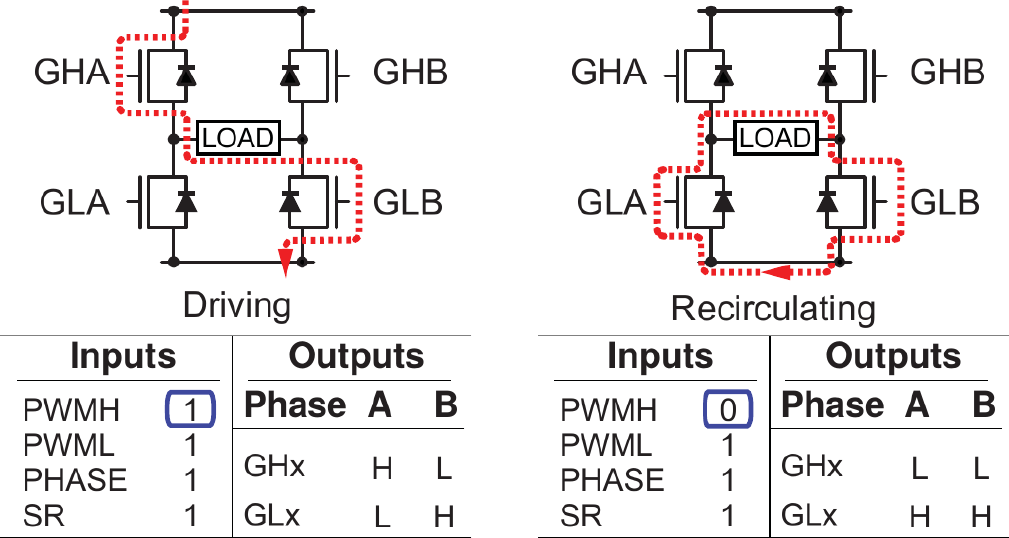
\includegraphics[width=.8\textwidth]{3941_2.png}\\
\caption{Slow decay, SR active, high-side PWM}%
\label{fig:3941_2}
\end{figure}

Konfiguration: PWML=1, PHASE=1, SR=1 und PWM an PWMH (high-side PWM)\\
Bei aktivierten PWMH fließt der Strom durch den GHA-Mosfets über den Motor und
dann über den GLB-Mosfet. in diesem Modus wird der Motor angetrieben.
Wenn PWML deaktiviert ist zirkuliert der vom Motor induziert Strom durch 
GLB und durch GLA, der Motor wird durch den niedrigeren Innenwiederstand des Mosfest 
stärker gebremst als in der Voherigen Konfiguration. Dabei ist darauf zu achten, dass
beinahe die gesamte induzierte Spannung über den beiden Mosfets (GLA/GLB) abfällt.
Was zu einer starken Hitzeentwicklung führen kann.



\begin{figure}[H]
\centering
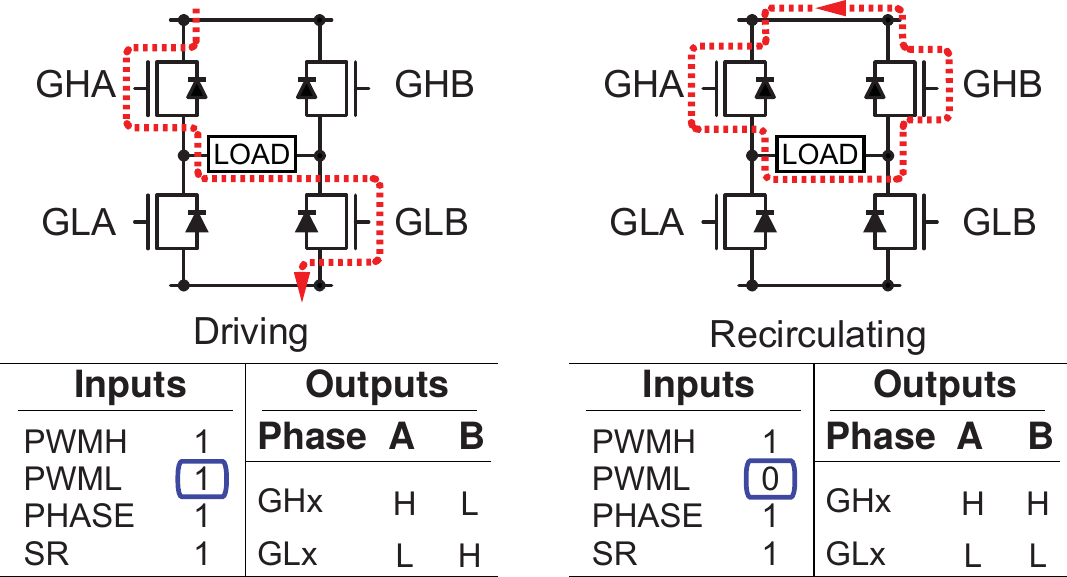
\includegraphics[width=.8\textwidth]{3941_3.png}\\
\caption{Slow decay, SR active, low-side PWM}%
\label{fig:3941_3}
\end{figure}

Konfiguration: PWMH=1, PHASE=1, SR=1 und PWM an PWML (low-side PWM)\\
Diese Konfiguration entspricht im Grunde den beiden vorherigen, Nur das dass PWM-Signal
an den unteren Mosfets anliegt. Der SR-Pin entscheidet wieder darüber ob im ``Bremsmodus''
die internen Dioden genutzt werden (SR=0) oder nicht (SR=1)




\begin{figure}[H]
\centering
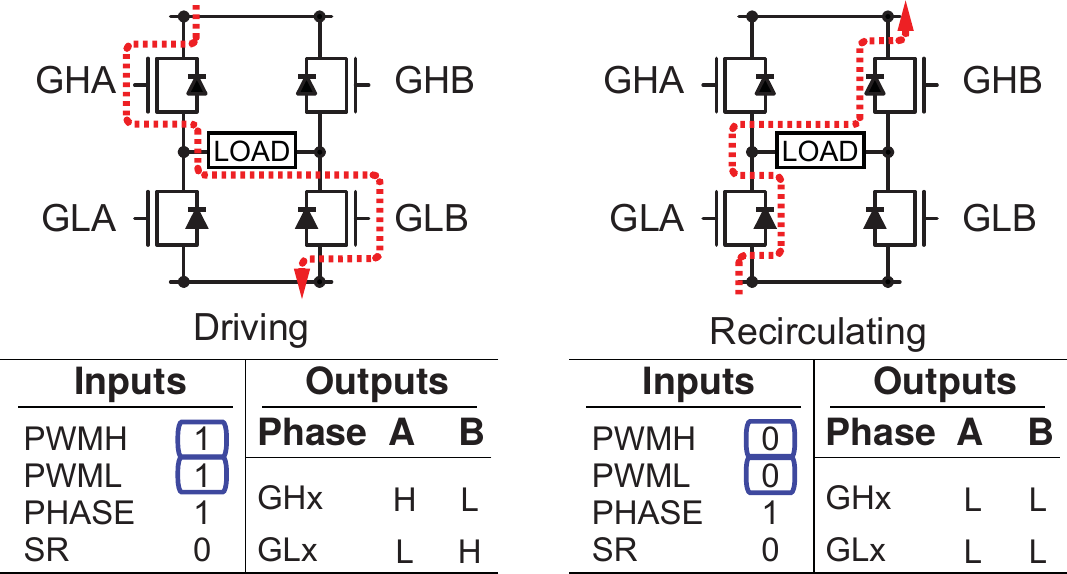
\includegraphics[width=.8\textwidth]{3941_4.png}\\
\caption{Fast decay, diode recirculation}%
\label{fig:3941_4}
\end{figure}


Konfiguration: PWMH=1, PWML=1, PHASE=1, SR=1\\
in dieser Konfiguration werden die oberen und unteren Mosfets gleich geschaltet. Im
``Bremsmodus'' führt das dazu das der induzierte Motorstrom nicht über die Mosfets
zirkulieren kann. Der Strom fließt stattdessen zurück in die Spannungsquelle, was
abhängig von der Spannungsquelle zu Schäden führen kann. Wird die Schaltung jedoch an
einem Akku betrieben ist es so möglich die Energie zu nutzen und damit den Akku
zu laden.

\begin{figure}[H]
\centering
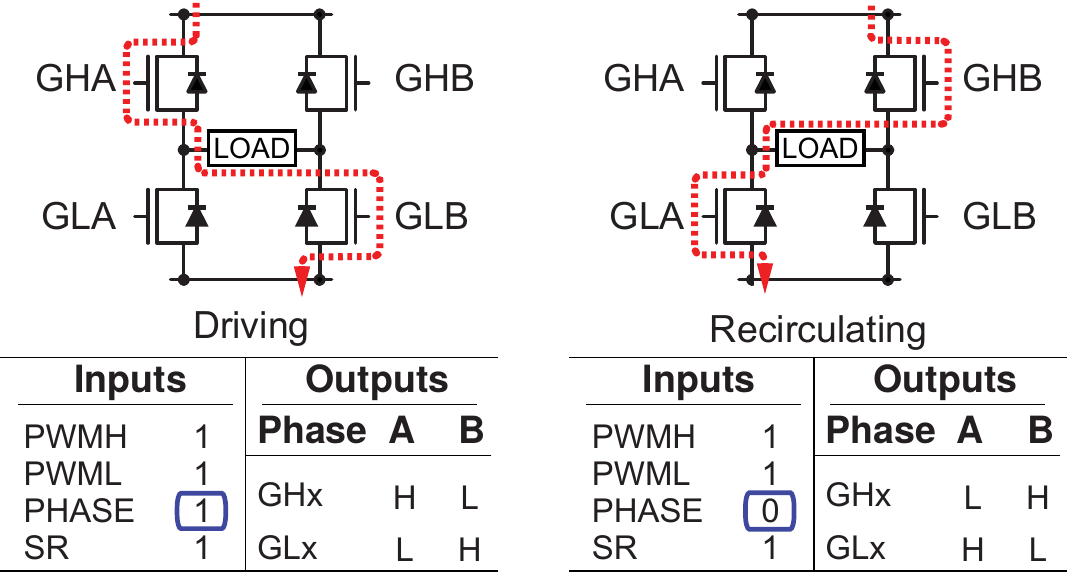
\includegraphics[width=.8\textwidth]{3941_5.png}\\
\caption{Fast decay, SR active, full four-quadrant control}%
\label{fig:3941_5}
\end{figure}

Diese Konfiguration zeigt den Einfluss des PHASE-Pins. Liegt am PHASE-Pin 1 ein an
fließt der Strom von links nach rechts. Liegt 0 an fließt er von rechts nach links.
Mithilfe des PHASE-Pins wird also die Polung des Motors festgelegt.

\section{Funk Empfänger}
Da die für die Funkkomunikationdas 2,4-GHz Frequenzband nicht genutzt werden darf können naheliegende Techniken wie W-Lan oder Bluetooth nicht genutzt
werden. 


\section{Beleuchtung}
Die einfachste Möglichkeit eine Beleuchtung am Auto zu realisieren sind Leuchtdioden, diese sind in allen erdenklichen Farben zu bekommen. Weiter Vorteile
sind das Leuchtdioden sehr Energieeffizient sind, außerdem sind sie zugünstigen Preisen zu bekommen. LEDs stellen keine großen Anforderugen an die 
Energieversorgung. Das Hauptproblem bei der Integration von vielen LEDs ist die Verkabelung. Eine große erleichterung bei der Integration sind 
LED-Streifen. Diese LED-Streifen gibt es in vielen Ausführungen. Für diese Arbeit interessant sind Allerdings nur jene Vertreter welche die Ansteuerung
jeder einzelnen LED zulassen. Die Ledstrips mit Chips von ``Worldsemi'' sind hierbei die prominentesten Vertreter. Zu erwähnen währen hierbei die Modelle
WS2801, WS2811 und WS2812. Der WS2812 ist dabei nahezu identisch mit dem WS2811 mit dem Unterschied, dass der WS2812 bereits in eine RGB-LED integriert ist.
Im unterschied zum WS2801 werden die beiden duche eine einzige Siganleitung mit fixem Takt angesteuert, so dass hier eine Seperate Taktleitung entfällt. Der Nachteil
an dieser Methode ist, dass die Timings genau eingehalten werden müssen um die Daten korrekt zu übertragen. Wie In Abbildung \ref{fig:led_cascade}werden die 
LEDs kaskadiert.Die Daten werden dann durch die LEDs geschoben.

\begin{figure}[H]
\centering
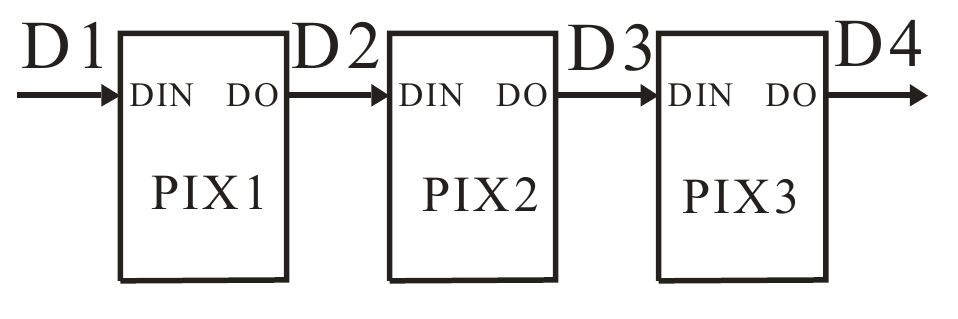
\includegraphics[width=.8\textwidth]{led_cascade.png}\\
\caption{Kaskadierung der LEDs}%
\label{fig:led_cascade}
\end{figure}

Um die beleichtung am Auto zu realisieren werden LEDs mit WS2812 genutzt. Die LEDs können an einem beliebigen
Eingang des AVR-Microcontrollers engeschlossen werden. Da die Timings exakt eingehalten werden müssen, ist die Software zur ansteuern in Assember geschrieben.
Jede LED wird mit einem 24Bit Datenwort angesprochen, dieses enthät die Helligkeitsstufen für jede der drei Grundfarben. Die Daten werden dabei
ohne Pause gesendet, bis alle LEDs im Strang die nötigen Daten erhalten haben. Nach jeder Übertragung muss eine Pause von mindestens 50\textmu s eingehalten
werden, damit die LEDs die Daten übernehmen. Die einzenen Bits der Übertragung sind dabei folgendermaßen codiert:

\begin{figure}[H]
\centering
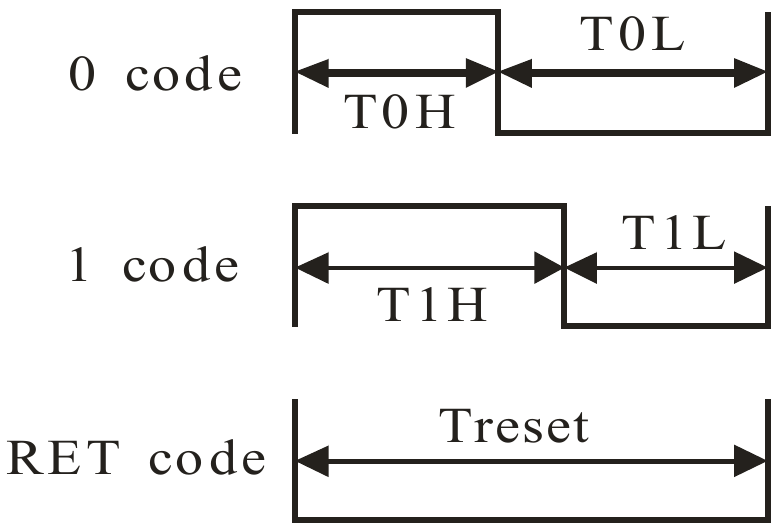
\includegraphics[width=.5\textwidth]{led_timing.png}\\
\caption{Codierung des LED Signals}%
\label{fig:led_timing}
\end{figure}

\begin{tabularx}{\textwidth}{|r|X|r|r|}
\hline
  Abschnitt & Beschreibung & Dauer & Abweichung \\ \hline
  T0H & 0 Code, high Zeit & $0.35\mu s$ & \textpm 150ns\\ \hline
  T1H & 1 Code, high Zeit & $0.7\mu s$ & \textpm 150ns\\ \hline
  T0L & 0 Code, low Zeit & $0.8\mu s$ & \textpm 150ns\\ \hline
  T1L & 0 Code, low Zeit & $0.6\mu s$ & \textpm 150ns\\ \hline
  RES & Reset Code, low Zeit & über $50\mu s$ & \\ \hline
\end{tabularx}


\section{Distanzsensoren}

 
\subsection{Messprinzip}
Die Ausgewählen Sensoren der Sharp GP2D Reihe basieren auf einer optischen Abstandsmessung. Geneauer der optischen Abstandsmessung durch Triangulation.
Bei der optische Abstandsmessung durch Triangulation projiziert ein Projktor einen Lichtpunkt auf das Messobjekt [\ref{fig:lasertriangulation}]. Ein optischer
Sensor misst dann den Winkel des vom Messobjekt reflektierten Lichtes. Durch Triangulation kann dann durch den fest definierten Abstand des optischen
Sensors von der Lichtquelle die Entfernung zum Objekt berechnet werden. \cite{Hugenschmidt2007}. In Abbildung \ref{fig:lasertriangulation} ist
diese Prinzipveranschaulicht
\begin{figure}[H]
\centering
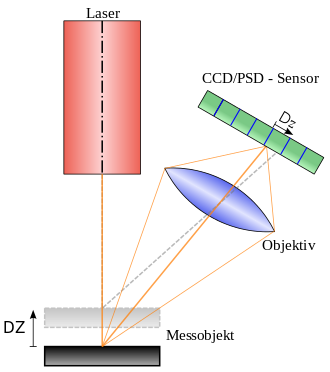
\includegraphics[width=.5\textwidth]{lasertriangulation.png}\\
\caption{Prinzip der Lasertriangulation}%
\label{fig:lasertriangulation}
\end{figure}

Vorteile des Messprinzips:
Da es sich um eine rein trigonometrische Messung handelt, kann sie zur kontinuierlichen Messung von Beweglichen Objekten verwendet werden.
Außerdem besitzen Sensoren nach diesem Prinzip einen kleinen Messfleck.

Nachteile:
Die Messung ist stark von der Oberläche des der Messobjktes abhängig, spiegelnde Oberflächen stellen ein großes Problem dar.
In Staubigen oder Nebligen Umgebungen wird das Lichtmöglicherweise zu früh reflektiert.

\subsection{Probleme der GP2D Sensoren}
Die Sensoren verfügen über einen analogen Ausgang. Bei analogen Signalen ist generell mit Störungen zu rechnen. Die GP2D Sensoren scheinen
hohe Anforderungen an die Energieversorgung zu stellen. Hier ist eine Entstörung mittels Kondensator von nöten da im Messignal sonst große Spikes
entstehen, wie in Abbildung \ref{fig:IR_spikes} zu sehen.

\begin{figure}[H]
\centering
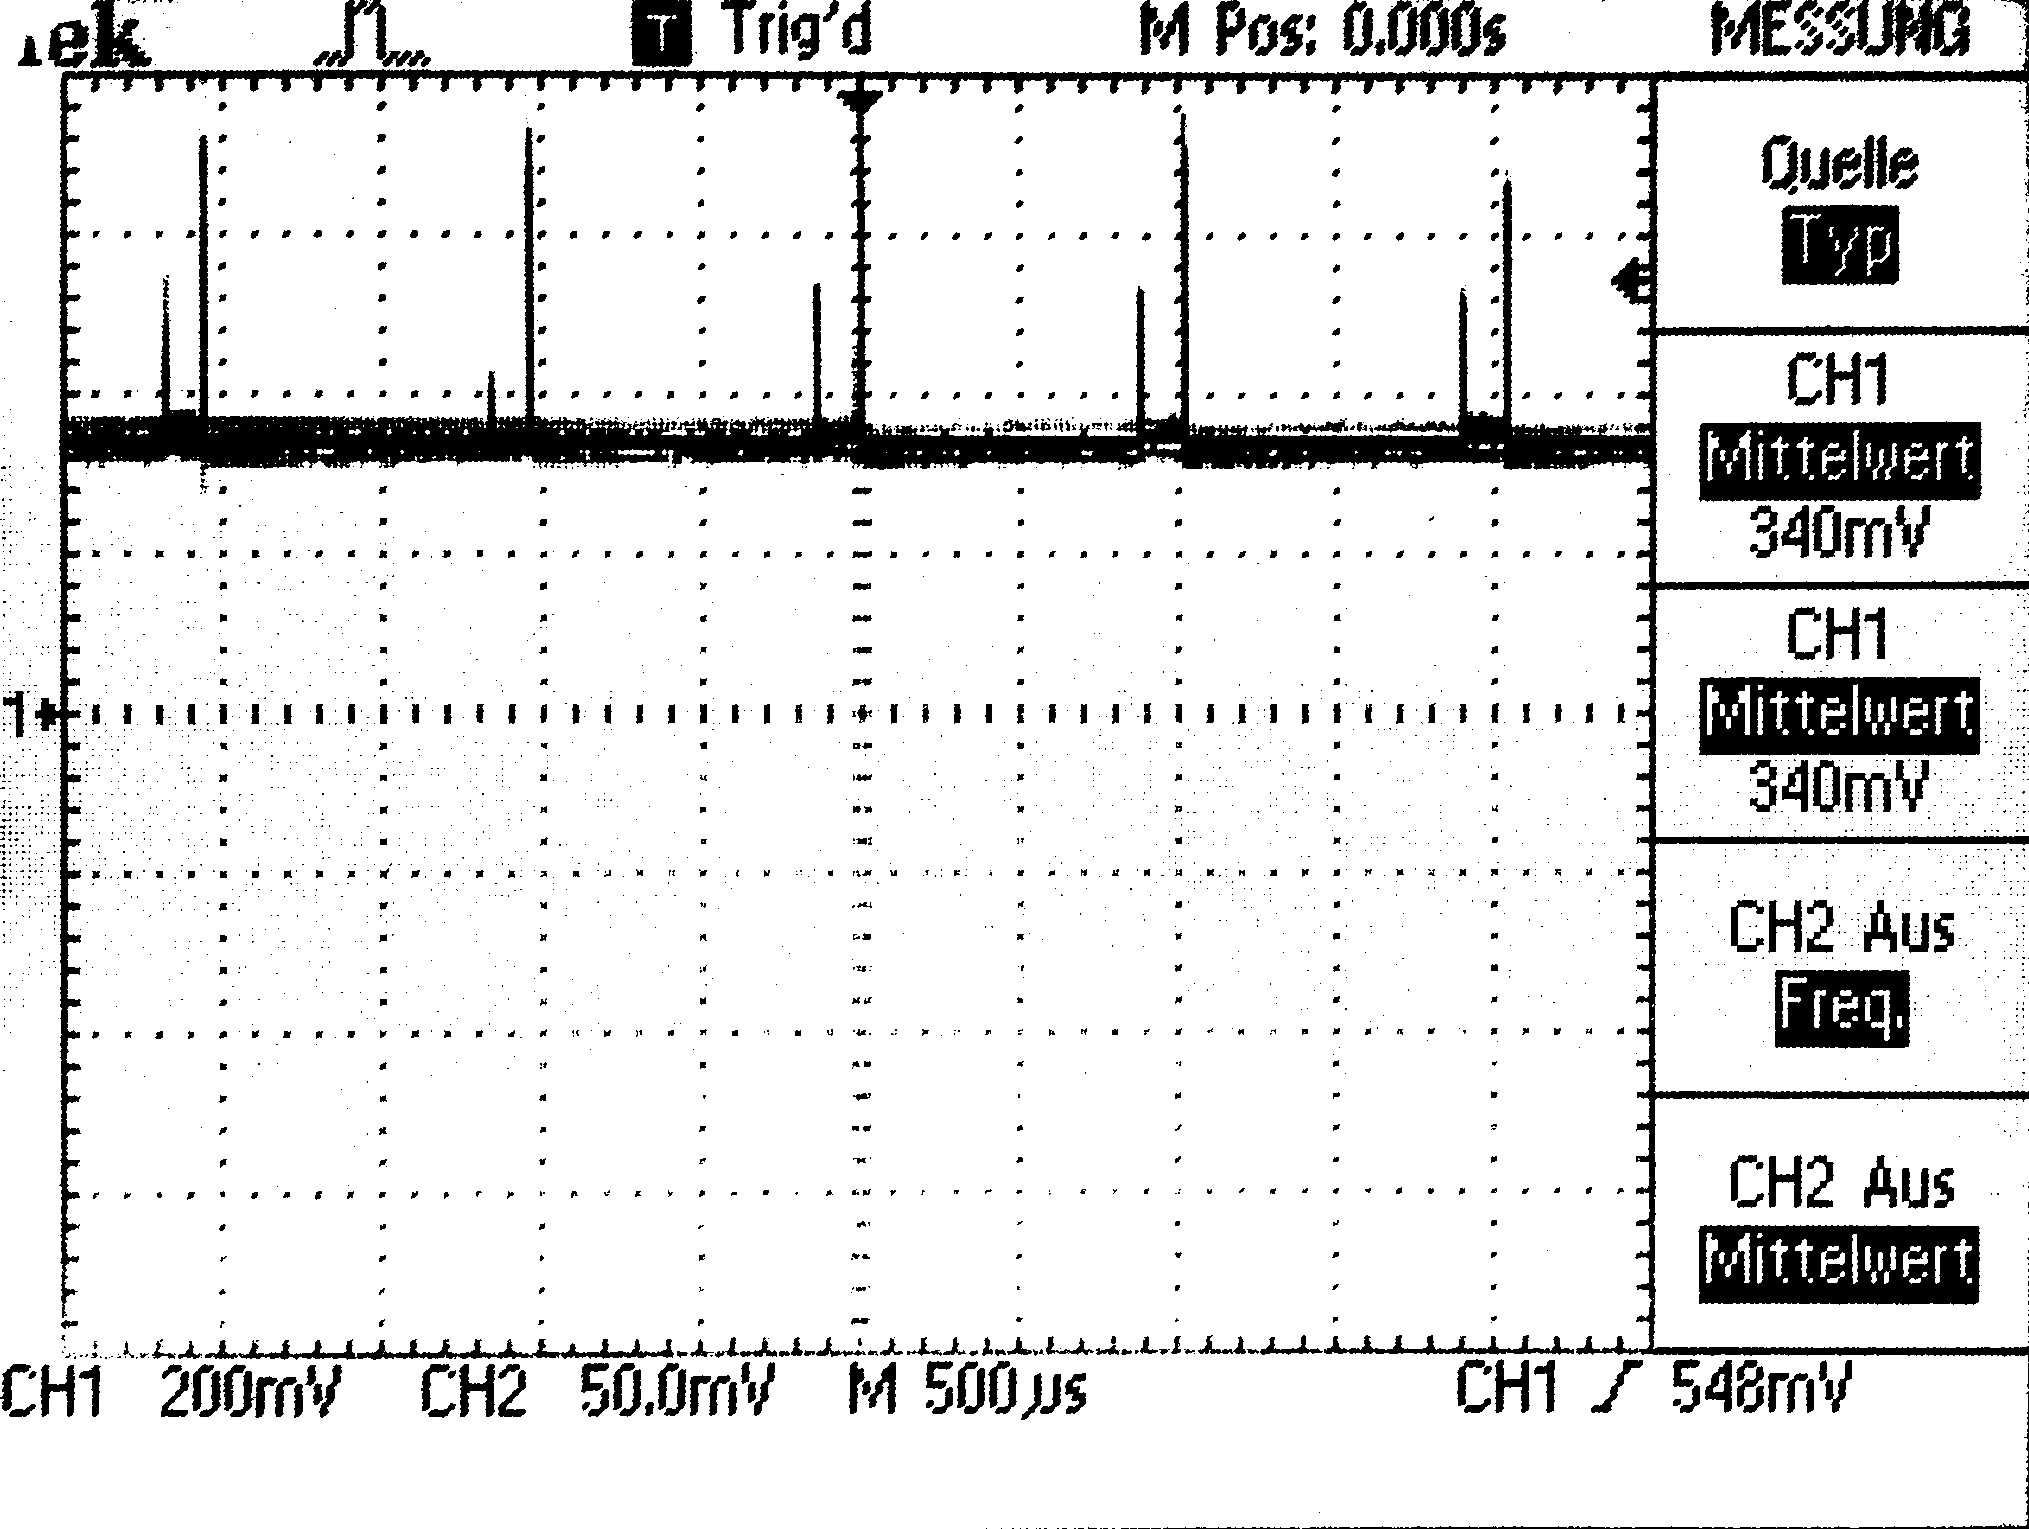
\includegraphics[width=.8\textwidth]{IR_spikes.png}\\
\caption{Ausgangssignal GP2D120}%
\label{fig:IR_spikes}
\end{figure}

Nach der Entstörung mit einem 82nF Kondensator direckt am Sensor zwiechen VCC und GND sind die Störungen bereits stark vermindert.

\begin{figure}[H]
\centering
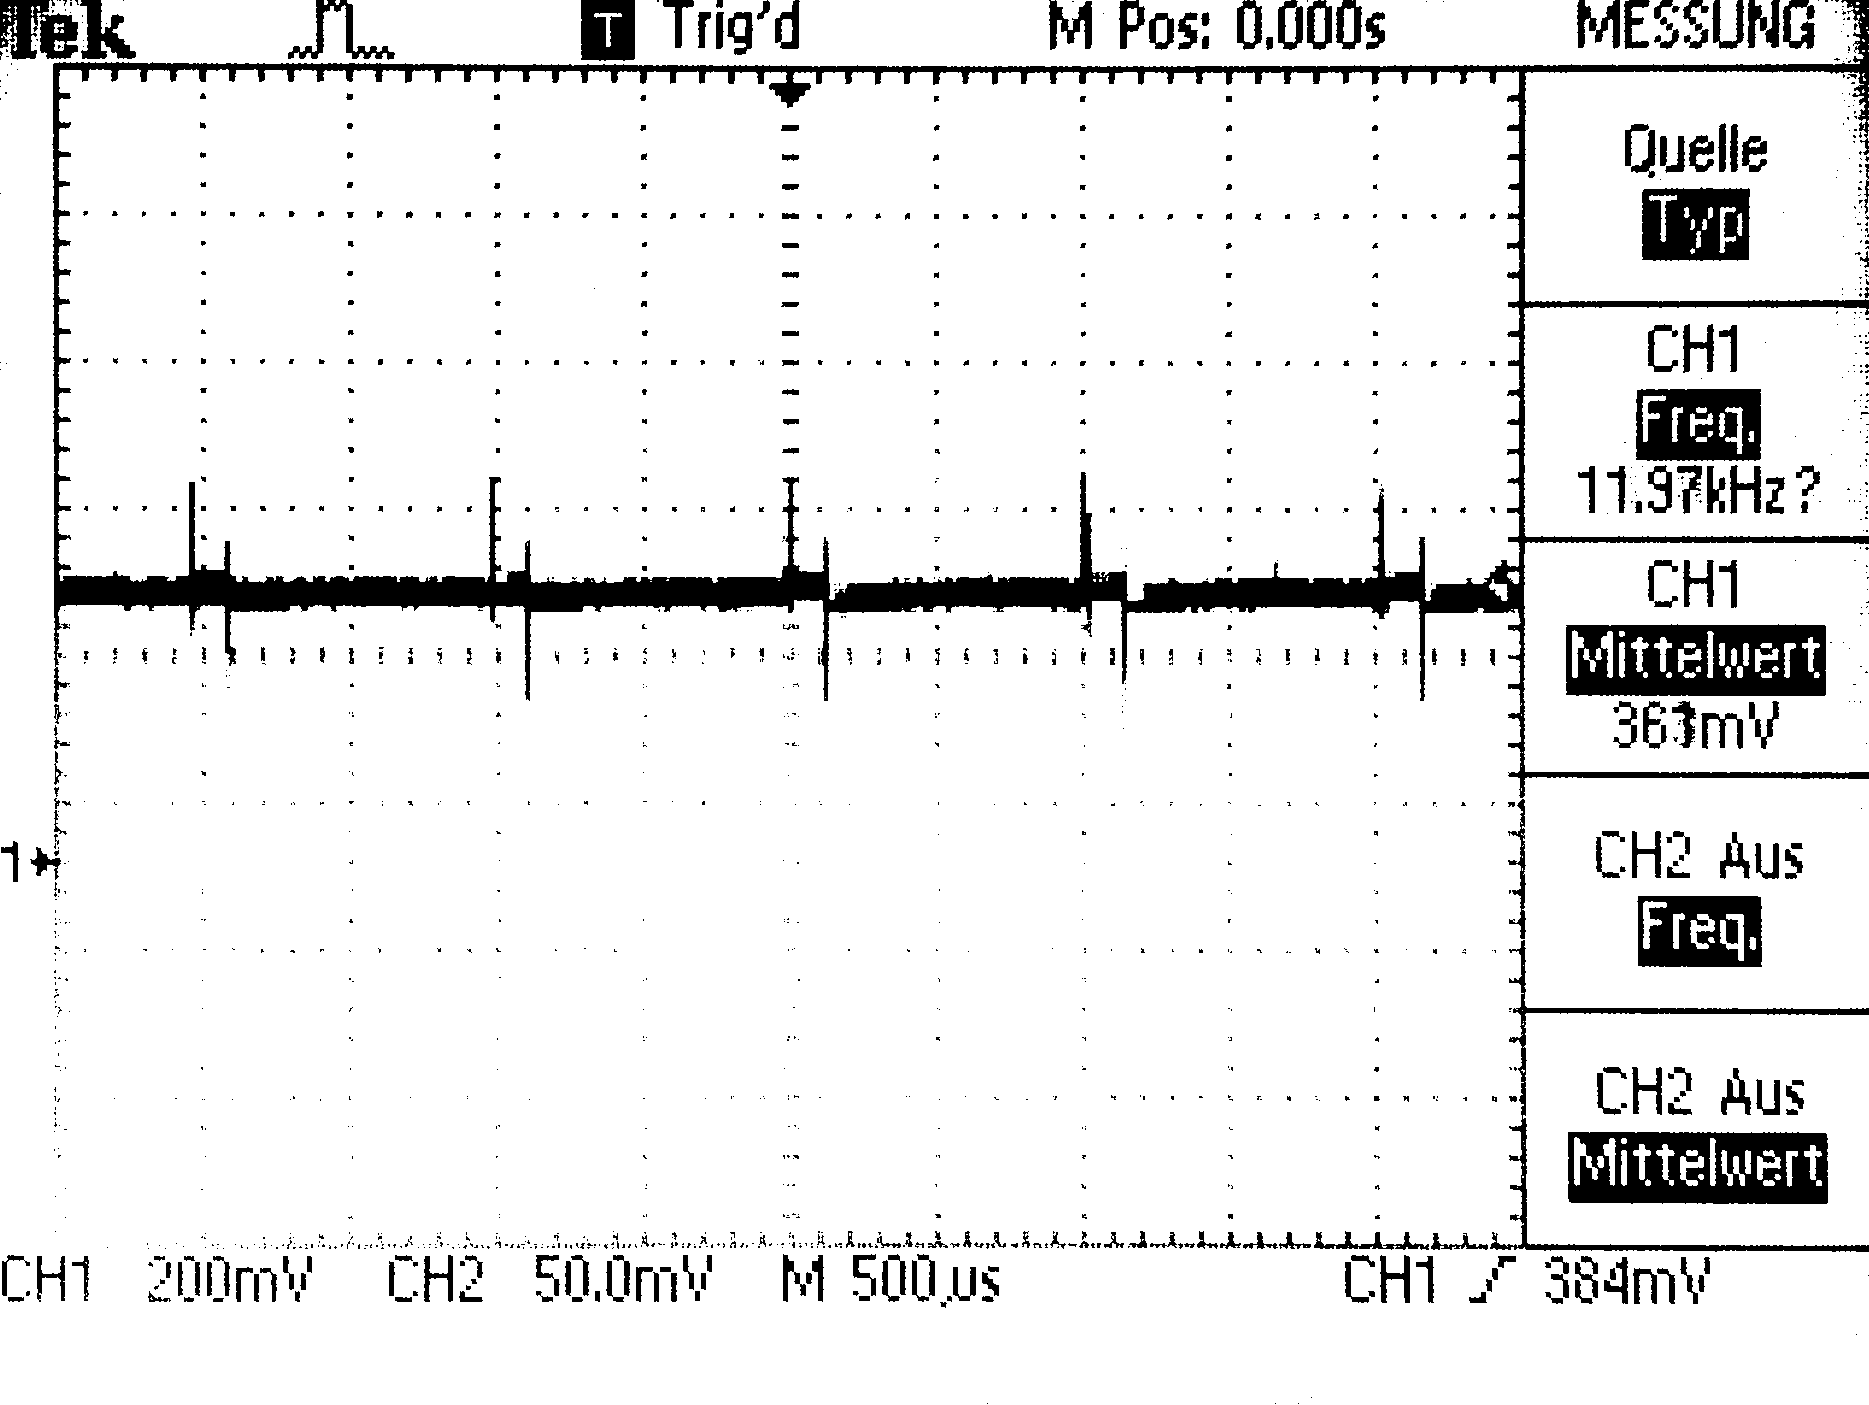
\includegraphics[width=.8\textwidth]{IR_lessspikes.png}\\
\caption{Ausgangssignal GP2D120 entstört}%
\label{fig:IR_lessspikes}
\end{figure}

\subsection{Auswertung des Messignales}
Das Messignal vom Sensor wird über einen ADC-Eingang des AVR Microcontrollers ausgelesen.



\section{Motor Derehzahlmessung}
Da Auto bentigt in unterschiedlichen Situationen unterschiedlich viel Leistung um seine Geschwidgkeit zu halten.
Besonders in Kurven ist durch die eröhte Reibung mehr Motorleistung nötig. Über den Motortreiber lässt sich jedoch nur
die Leistung am Motor verändern, deshalb ist es nötig diese zu Regeln. Dafür ist jedoch eine Rückführung der Geschwindigkeit
des Autos nötig. Eine Aufintegrierung der beschleunigungs Daten der Interialsensorik führt auf dauer leider zu erheblichen
Abweichungen und ist daher für eine Regelung nicht geeignet. Leider ist auch eine Odometrie an den Rädern des Autos
aus mechanischen Gründen schwer zu realisieren. 
\subsection{Hallsensor}
Duch die feste Übersetzung des Getriebes bietet die Messung der Motordehzahl
eine gute Nährung für die aktuelle Geschwindigkeit. Eine Moglichkeit die Motordrehzahl zu messen ist es das Magnetfeld des
Motorankers auszuwerten. Dazu sehen wir uns den Aufabu eines Gleichstommotors an.
\begin{figure}[H]
\centering
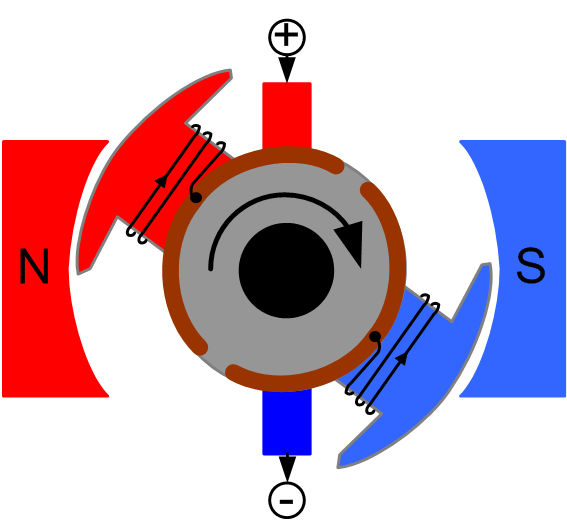
\includegraphics[width=.5\textwidth]{motor.png}\\
\caption{Aufbau eines Gleichstommotors}%
\label{fig:lasertriangulation}
\end{figure}
Ein Gleichstommotor besteht aus Zwei Grundsätzlichen Teilen, einem unbeweglichen Teil, den Stator und einem beweglichen Teil, dem Anker.
Der Stator besteht aus sich gegenüberliegenden Permanentmagneten welche Zwei entgegengesetzt gepolte Magnetfelder erzeugen.
Der Anker besteht aus Elektromeganeten dessen Polung jede halbe Umdrehung kommutiert wird. Duch die kommutierung ändert sich die 
Polung der Elektromeganeten. Das sich so änderne Magnetfeld kann mit einem Hallsensors ausgewertet werden. Das so entstehende 
Signal ähneld dabei über der Zeit einer Sinusschwinnung. Mit Hilfe eines Schmitt-Trigger kann daraus ein Drehzahlsignal generiert werden.

Der Hallsensor ist erfolgreich durch ein Belüftungsloch im Motor plaziert werden. Als Referenzspannung für den Schmitt-Trigger wird der
Mittelwert des Sensorsignals, erzeugt durch einen Tiefpass, genutzt.

\begin{figure}[H]
\centering
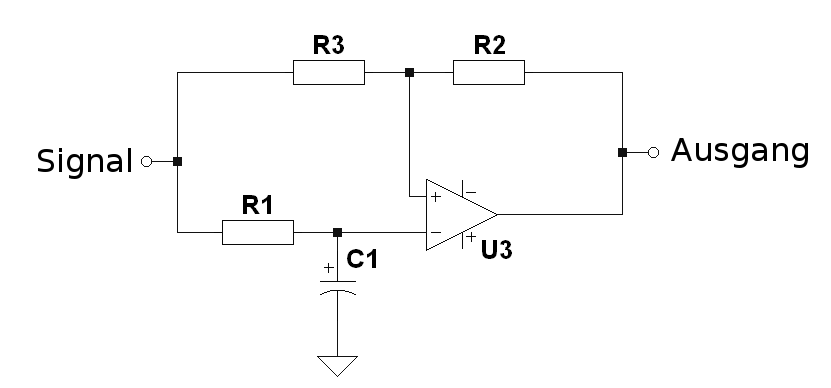
\includegraphics[width=.5\textwidth]{schmitt.png}\\
\caption{Schmitt-Trigger Schaltung}%
\label{fig:schmitt}
\end{figure}

Leider führt dieses Vorgehen nicht zum Erfolg, da die Megnetfeldstärke stark von der Drehrichtung des Motors abhängt. Es war ist möglich
den Schmitt-Trigger so auszulegen, das er in beide Drehrichtungen zuverlässig funktioniert. Alternativ zu diesem vorgehen gibt es
andere Lösung. Eine Speziell für diesen Motor angefertigte Achsverlängerung wird eine Inkrementalgeberscheibe befestigt. Diese wird durch einen
Sharp GP1A30R Sensor ausgewertet und liefert ein Drehszahlsignal an den externen Takteingang des Timer 1 vom AVR Microcontroller.


  
\section{Motorstrommessung am Shunt}


\subsection{Problem}

An einem mit PWM angesteuertem DC-Motor soll eine Strommessung mit Hilfe eines Shuntwiederstandes
durchgeführt werden. Aufgrund der PWM Ansteuerung muss der DC-Anteil aus dem Signal herausgefiltert werden!


\subsection{Prinzip der Strommessung}

Die Messspannung wird über einen Shuntwiederstand zur Masse gemessen! Aufgrund nicht vorhandener Datenblätter des Motors
wird von einem expirimentel Ermittelten maximalen Strom des Motors ausgegangen. Dieser beträgt bei einer Betriebsspannung von 20V ca. 20A.
Da einen Shunt mit einer maximalen Belastbarkeit von 2 Watt eingesetzt wird, darf der maximale Spannungsabfall am Shunt 100mV nicht überschreiten.
Nach dem Ohmschen Gesetz ergibt sich dadurch ein Widerstand von $0,005 \Omega$  für den Shunt. Shuntwiederstände in der Größe sind problemlos zu bekommen.
Da es sich hier um eine Worst Case Rechnung handelt, wird der zusätzliche Widerstand des Shuntwiederstandes und der damit verringerte Strom bewusst ignoriert.

Die über den Shuntwiederstand gemessene Spannung soll über den ADC Eingang des Mikrocontrollers eingelesen werden. Vorher jedoch muss das Signal gefiltert werden, da der Strom
durch die Ansteuerung mittels der Pulsweitenmodulation nicht konstant ist!



\subsection{Anforderungen}
Die maximale Auflösung des Mikrocontrollers soll ausgenutzt werden. Der ADC des Mikrocontrollers arbeitet mit einer Auflösung von 10 Bit und einer 
Referenzspannung von 5V. Um die Auflösung des ADC auszunutzen muss das Signal, aufgrund unseres Spannungsabfalls verstärkt werden.

Als Anforderung ergibt sich außerdem, dass der maximale Ripple des Endsignals kleiner ist als der Quantisierungsfehler des ADC.
So ist es möglich aufeine zusätzliche digitale Filterung weitgehend zu verzichten.
Die kleinst mögliche zu erfassende Spannung des ADC beträgt $\frac{5}{2^{10}}=4,88mV$.
Diesen wert sollte der Ripple des Endsignales nicht überschreiten.
Aus einem möglichst kleinem Ripple resultiert eine möglichst hohe Filterordnung bzw. eine niedrige Grenzfrequenz.
Allerdings soll $U_{DC}$ einer Änderung des Mittelwertes, also einer Änderung des Tastverhältnisses, möglichst
schnell folgen. Diese Anforderung widerspricht der Vorherigen, so das ein Kompromiss gefunden werden muss.

\subsection{Bestimmung des Filtertyps}
Aufgrund des sehr niedrigen Spannungspegels am Shunt,ist es nötig das Signal zu verstärken. Da zum verstärken des Signals aktive elektronische Elemente notwendig sind,
z.B. ein Operationsverstärker, wird an dieser Stelle gleich ein aktiver Filter verwendet. Dieser gibt uns die Möglichkeit des Messignal zu verstärken und gleichzeitig zu
Filtern. Da wir als unser Signal im optimalen Fall eine Gleichspannung darstellt müssen wir die Hochfrequenten Anteile unseres Signales herausfiltern, dies geschieht 
mit Hilfe eines Tiefpasses. Es gibt im Grunde 2 übliche aktive Tiefpässe, den Tiefpass mit Mehrfachgegenkopplung und den Sallen-Key Filter. Ersterer verwendet
einen invertierenden Verstärker, dieser invertiert das Messsignal. Da der \textmu Controller jedoch nur mit positiven Spannungen umgehen kann müsste man hier mit einer 
negativen Referenzspannung Arbeiten, was den Schaltungsaufwand unnötig vergrößern würde. Der Sallen-Key Tiefpass benutzt einen nicht invertierenden Verstärker, welcher diesen
Nachteil nicht hat. So dass ab dieser Stelle ein Sallen-Key Tiefpass entwurfen wird.

%%TODO Quellen (verweise auf übliche Filtertypem)

\subsection{Die Filterschaltung}

wie im vorherigen Abschnitt diskutiert wird hier ein Sallen-Key Tiefpass entwurfen. Zum Entwurf der Schaltung wurde Eagle genutzt.

\begin{figure}[H]
\centering
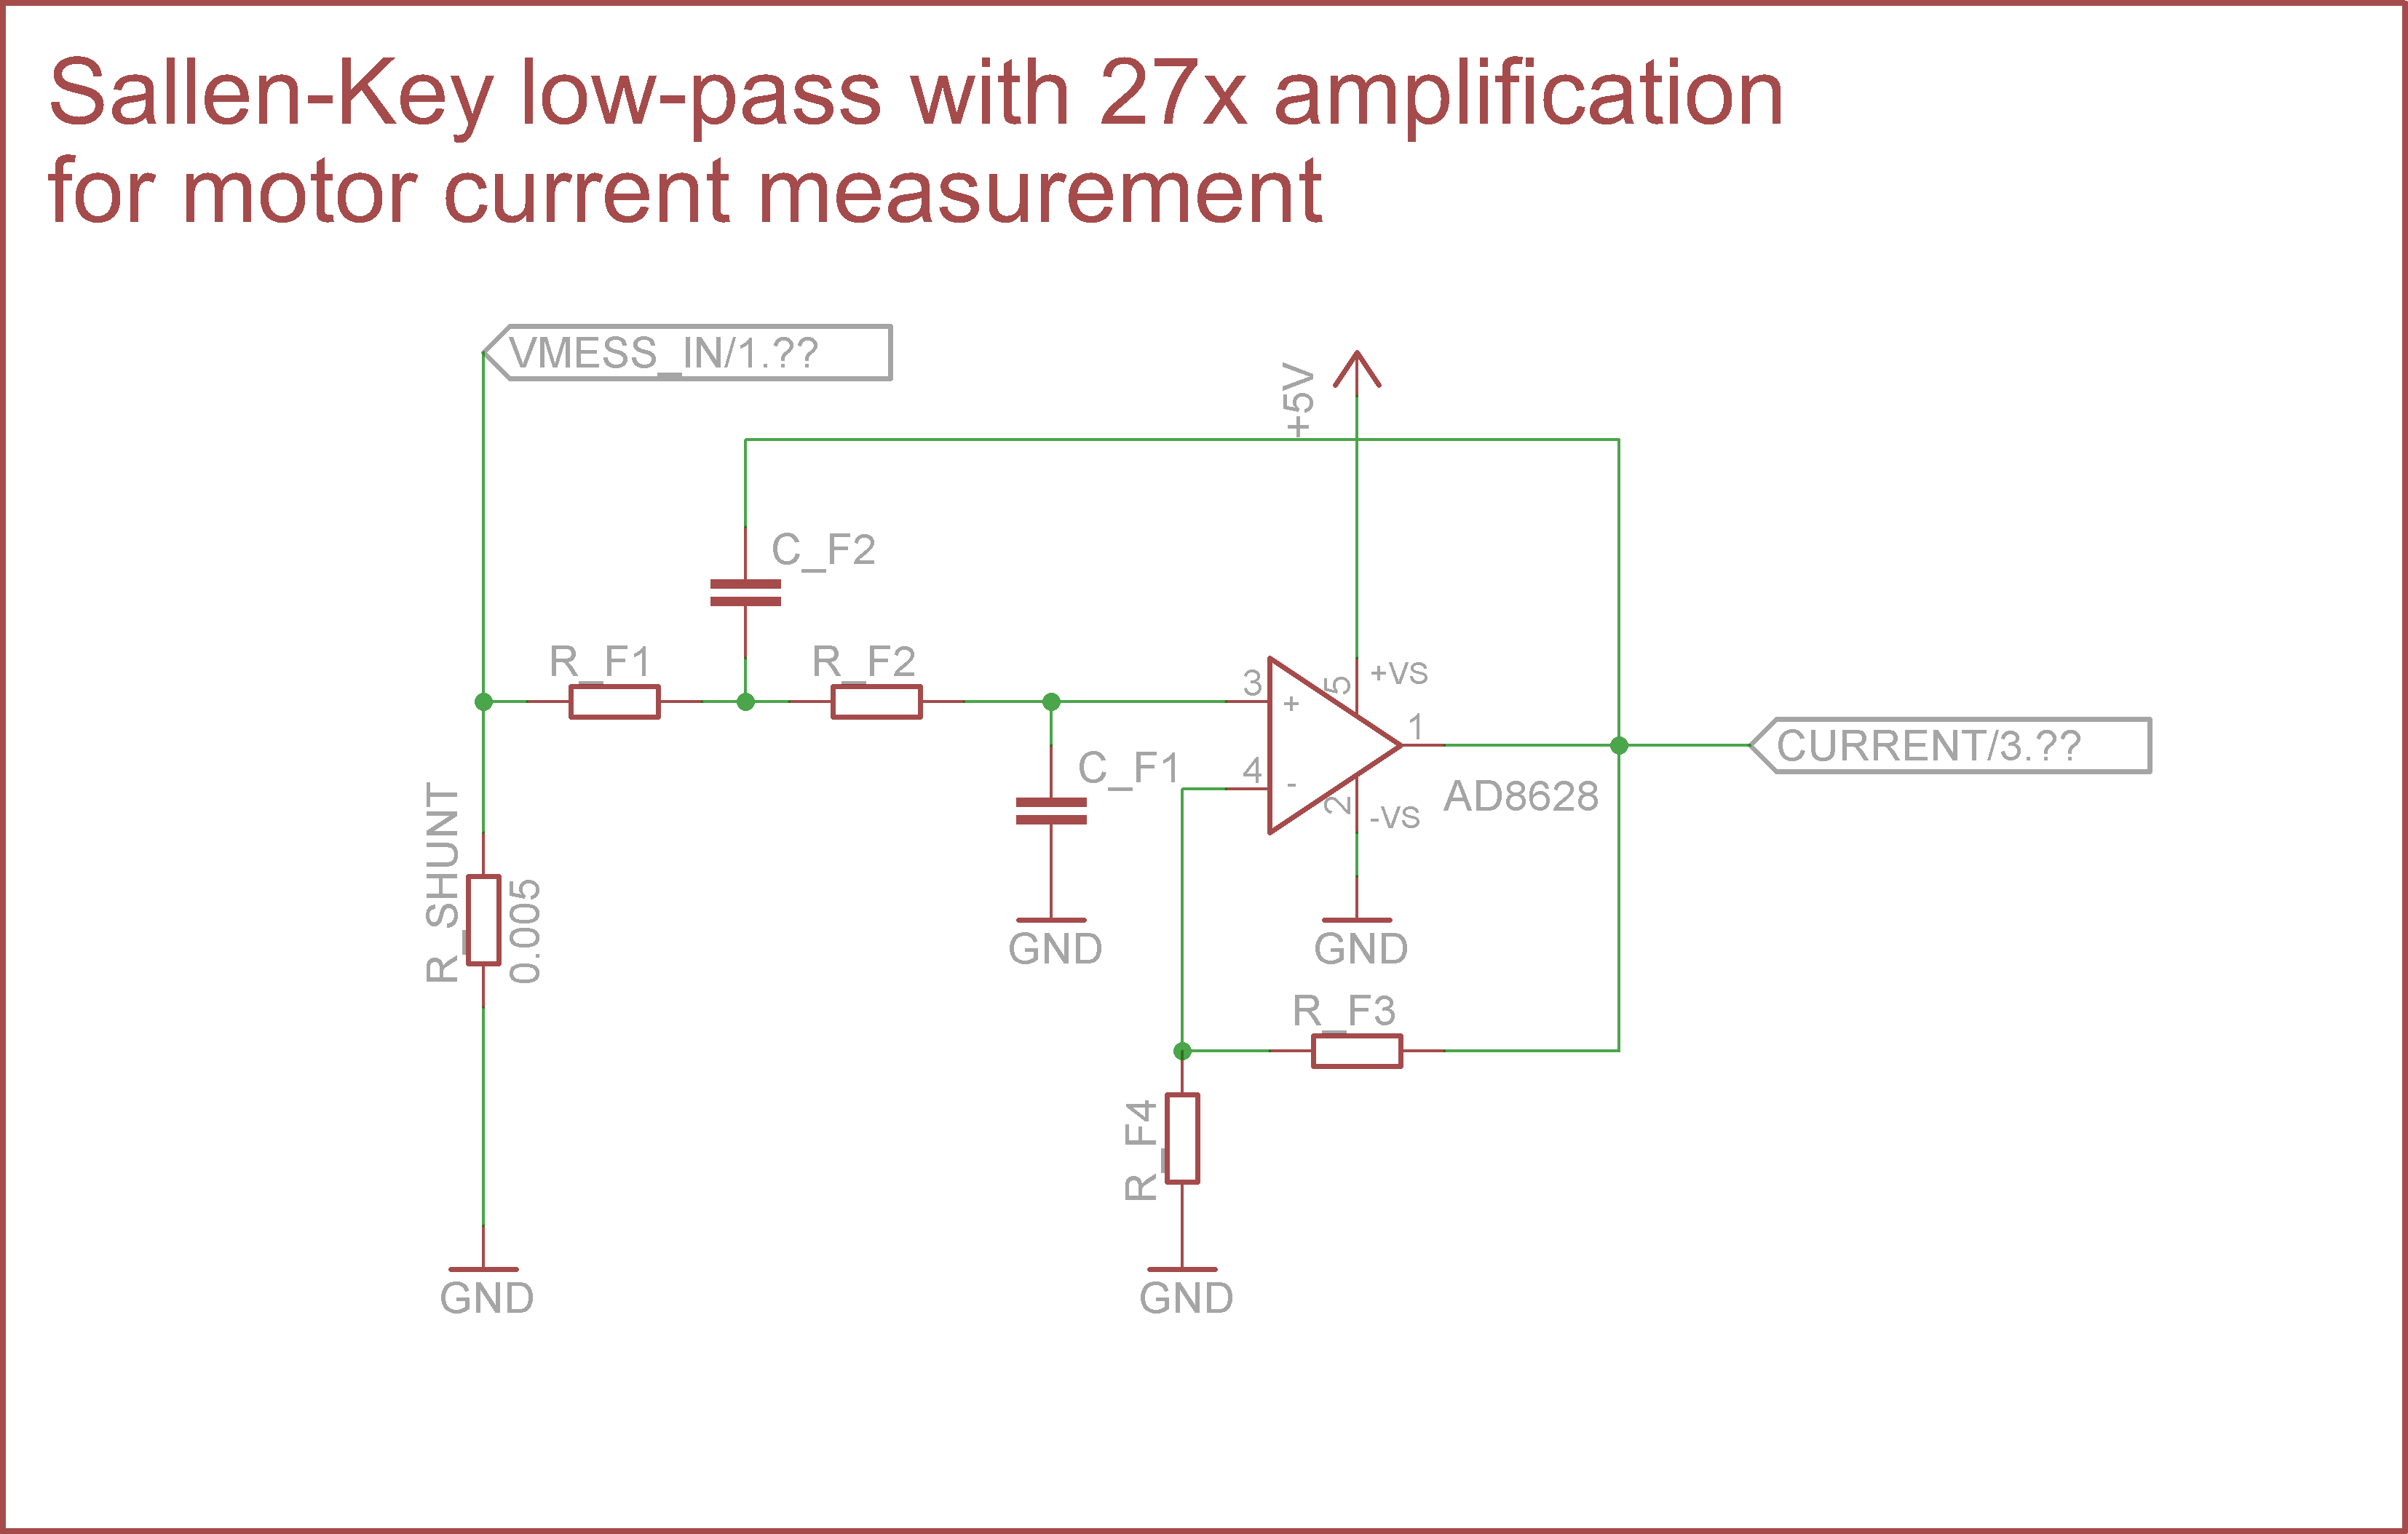
\includegraphics[width=.8\textwidth]{filter_schaltung.png}\\
\caption{Salle-Key Tiefpass mit Shunt}%
\label{fig:fschalt}
\end{figure}



\subsection{Dimensionierung des Verstärkers}

In bisherigen Rechnungen wurde ein maximaler Spannungsabfall von 100mV am Shunt errechnet. Da der Messbereich des voll ADC ausgenutzt werden soll,
ist es nötig das Messsignal zu verstärken. Hierzu wir ein Nichtinvertierender Verstärker benutzt. Da der Messbereich des ADC bis 5V reicht, wird hier eine 
50 fache Verstärkung angestrebt.

Für einem Nichtinvertierenden Verstärker ergibt sich dann:

\begin{align*}
v &= 1 + \frac{R_{F3}}{R_{F4}}\\
50 &= 1 + \frac{R_{F3}}{R_{F4}}\\
49\cdot R_{F4} &= R_{F3}
\end{align*}
\\
Wobei $R_{F4} = 47 k\Omega$ und $R_{F3} = 1 k\Omega$  gewählt werden, was eine Verstärkung von 48 ergibt.

%%TODO Warum werde widerstände so gewählt

\subsection{Anforderungen an den Filter}

\begin{figure}[H]
\centering
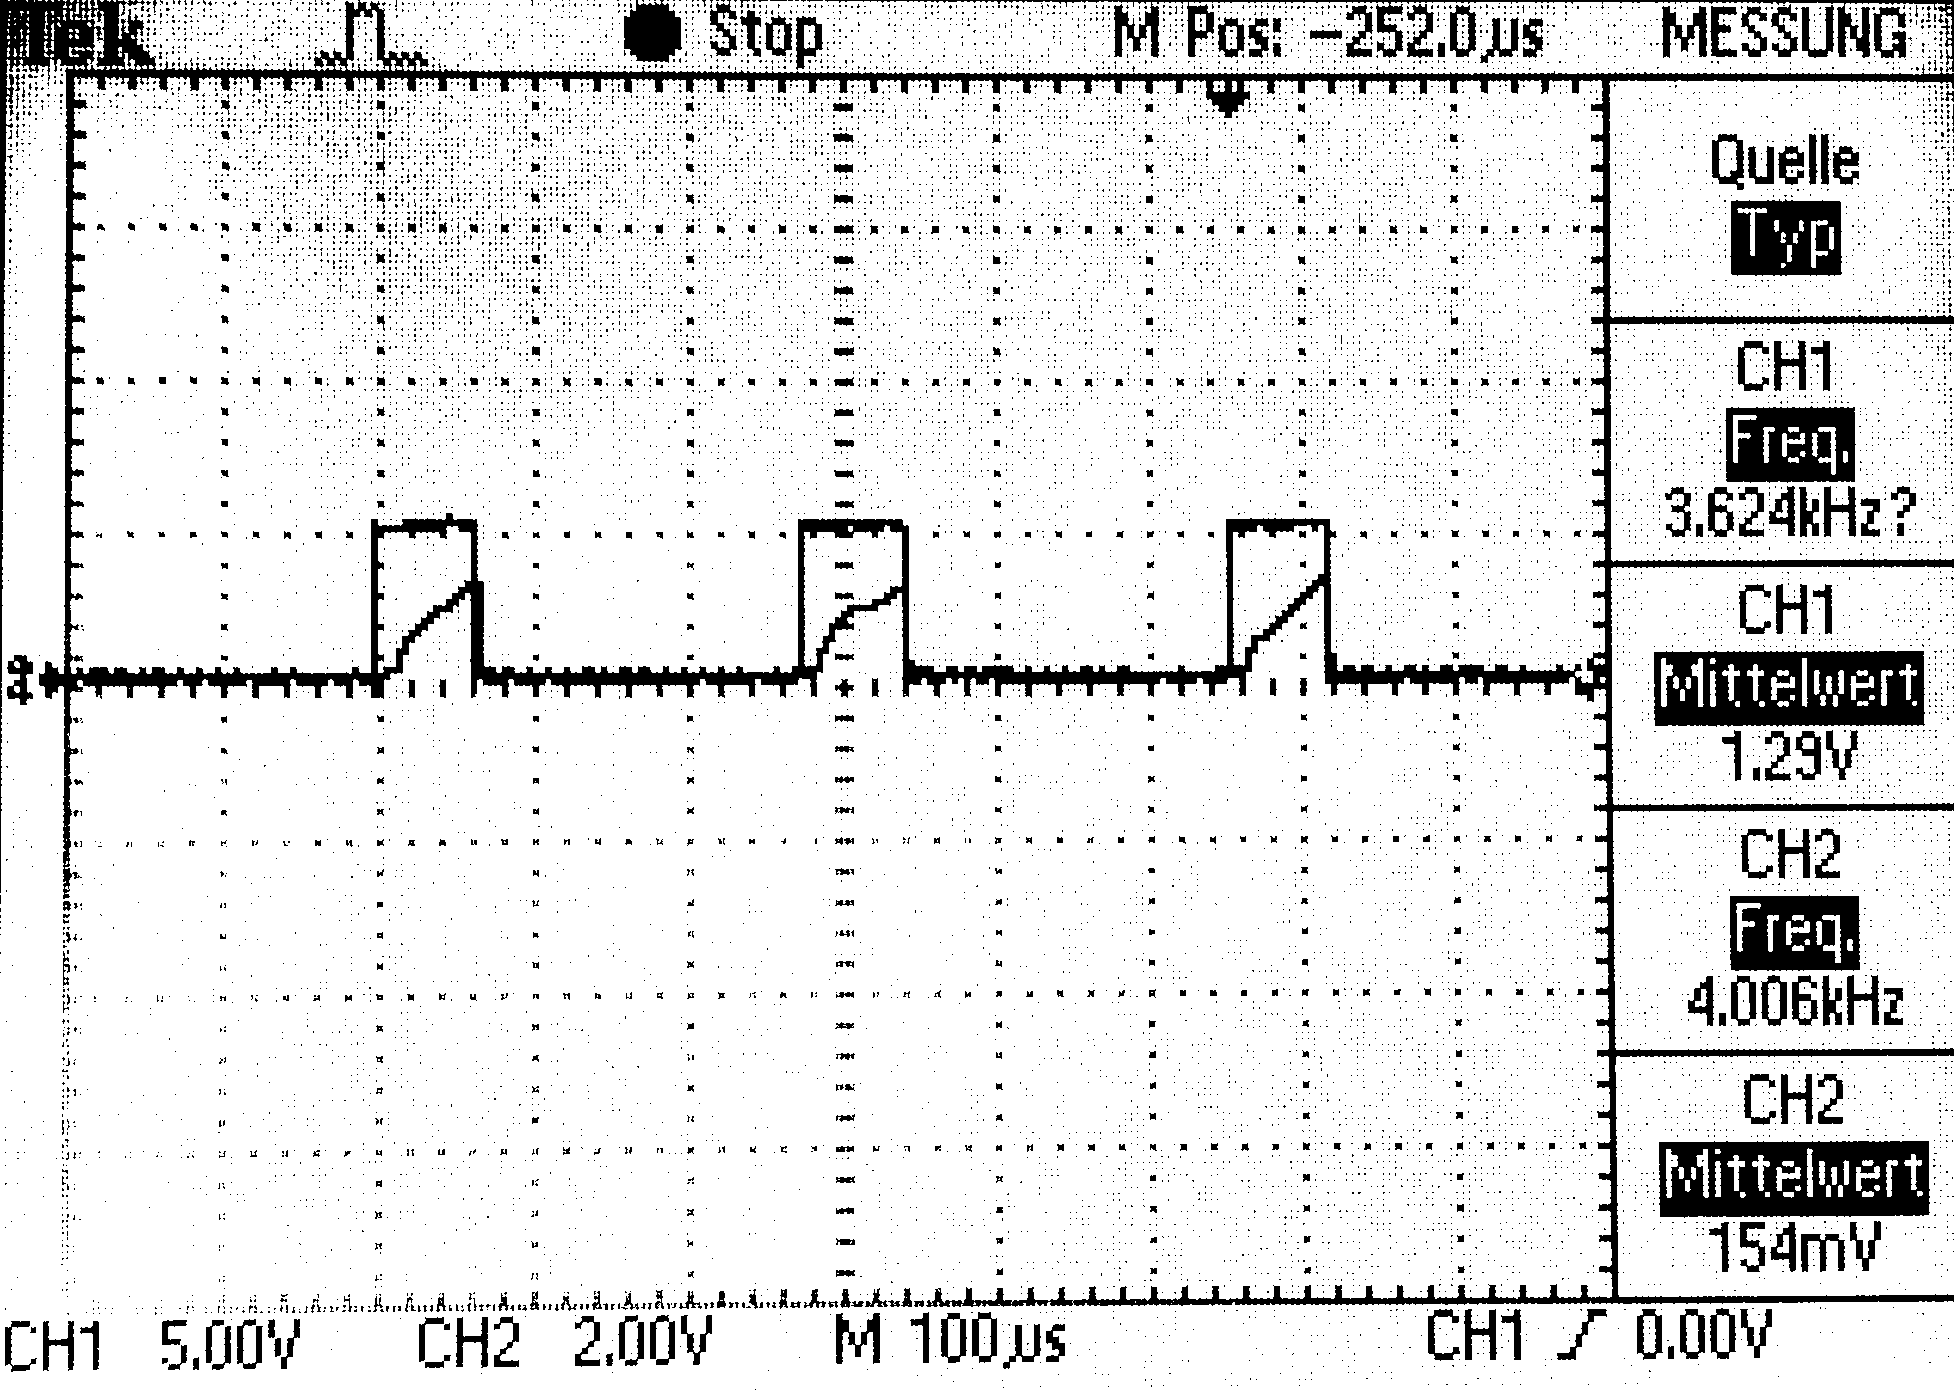
\includegraphics[width=.8\textwidth]{oszi.png}\\
\caption{Spannung am Shunt + PWM}%
\label{fig:pwm+i}
\end{figure}

Da dem Messsignal wie in Abbildung \ref{fig:pwm+i} zu erkennen, die PWM Frequenz zu Grunde liegt wird sich bei der Dimensionierung des Filters einer Idee nach \cite{Alter2008} bedient, nach der die maximale Amplitude des Ripple der Grundschwingung bei einem
Tastverhältnis von 0,5 entspricht. Die Amplitude der Grundschwingung ergibt sich aus dem ersten Koeffizienten der Fourierreihe einer Rechteckschwingung.
\begin{align}
A_1 = K\cdot \frac{1}{\pi}[\sin(\pi p)-\sin(2\pi(1-\frac{p}{2}))]
\label{eq:ripple}
\end{align}
Wobei $p$ dem Tastverhältnis und $K$ der maximale Amplitude des Ursprungsingals entspricht \cite{Alter2008}. $K$ entspricht den errechneten 100mV multipliziert mit dem Verstärkungsfaktor 48, also 4,8V. Das Tastverhältnis $p$ wird zu 0,5
angenommen. Mit (\ref{eq:ripple}) ergibt sich für die Amplitude der Grundschwingung $ A_1 = K\cdot \frac{2}{\pi} = 3,056V$. $A_1$ soll auf $ < 4,88mV$ gedämpft werden.
Als Sperrfrequenz $\Omega_s $ wird hier die PWM Frequenz angesetzt. Für $H(\omega=2\pi f_{PWM})$ gilt also:

\begin{align}
H(\omega=2\pi f_{PWM}) \le \frac{4,88mV}{3,056V} \mathop{\hat{=}} 20\cdot\log(\frac{4,88mV}{3,056V})= -55,9 dB
\label{eq:daempfung}
\end{align}

Da das Projekt möglichst kostensparend durchgeführt werden soll, also auch Bauteilsparend, wird im Folgenden von den üblichen Konventionen zur dimensionierung von Filtern abgewichen.
Statt eine fixe Grenzfreqeunz festzulegen und die benötigte Filterordnung zu bestimmen, wird die Filterordnung vorgegeben und die Grenzfrequenz variiert.

\subsection{Filterentwurf}

\subsubsection{Bestimmung des Filtertyps}

Des Filtertyp muss in zweierlei Hinblick bestimmt werden. Einmal im hinblick auf die Schaltung und seinem Frequenzgang.
Im groben gibt es 2 mögliche aktive Tiefpassfilterschaltungen, den Sallen-Key Teifpass mit nicht invertierendem OPV und dem aktiven Tiefpass mit Mehrfachgegenkopplung 
(invertierender OPV). Der aktive Tiefpass mit Mehrfachgegenkopplung benötigt allerdings negative Spannungsniveaus die auf der Treiberplatine nicht zur
verfügung stehen, deshalb wird an dieser Stelle nur der Sallen-Key Teifpass betrachtet.
Was den Frequenzgang angeht gibt es viele Filtercharakteristiken, eine Auswahl an haufig verwendeten Charakteristiken wird hier verglichen.

Der \emph{Butterworth}-Filter besitzt einen maximal flachen Verlauf des Frequenzganges im Durchlassbereich und eine monoton verlaufende Dämpfung im Sperrbereich.
Leider hat der Butterworth-Filter nur eine geringe Flankensteilheit im Sperrbereich (20dB/Dekade pro Ordnung). Ein Butterworth-Filter 1. Ordnung entspricht einen  einfachen RC-Filter.

Der \emph{Tschebyscheff}-Filter hat eine höhere Flankensteilheit als der Butterworth-Filter, allerdings entsteht beim Tschebyscheff-Filter Welligkeit im Durchlassbereich,
welche mit höherer Ordnung zunimmt. Durch die Welligkeit im Duchlassbereich würde ein zusätzlicher Ripple im Signal entstehen, weshalb der Tschebyscheff-Filter nicht
für den geforderten Filter geeignet ist 

Der \emph{Bessel-Filter} hat den Vorteil einer konstanten Gruppenlaufzeit, hat dafür aber eine noch geringere Flankensteilheit als der Butterworth-Filter.
Da eine konstante Gruppenlaufzeit für den geforderten Filter nicht von Vorteil ist, da das Endsignals einer Gleichspannung entsprechen sollte, ist der Butterworth-Filter
die bessere Wahl.


\begin{figure}[H]
\centering
\begin{tikzpicture}
	\draw[->,thick] (0,0) -- (7.5,0) node[right] {$f[\text{Hz}]$};
	\draw[->,thick] (0,0) -- (0,3.3) node[above] {$a[\text{dB}]$};
	\draw (0,2.5)node[left] {$a_{\text{min}}$} (-0.1,2.5)--(2.9,2.5);
	\draw (0,1)node[left] {$a_{\text{max}}$};
	\def \bsp{(0,1)--(1,1)--(1,2.4)--(1,2.4)--(0,2.4)}
	\draw (-0.1,1)--(1,1)--(1,2.4) (1,0)node[below] {$f_g$};
	\pattern[pattern=north east lines] \bsp;
	\draw[dashed] (1,1) -- (1,-0.1);
	\def \bsd{(3,0) -- (3,2.5) -- (7,2.5) -- (7,0)}
	\pattern[pattern=north east lines] \bsd;
	\draw (3,0)node[below] {$f_s$} -- (3,2.5) -- (7,2.5);

\end{tikzpicture}
\caption{Tiefpass Toleranzfeld}%
\label{fig:analog}
\end{figure}
Für unsere Schaltung wird ein Sallen Key Tiefpass 2. Ordnung entwurfen. Die PWM-Frequenz $f_{PWM}$ beträt 3,9kHz.
Die Sperrfrequenz entspreicht der PWM Frequenz, also der Frequenz unserer Grundschwingung. $\Omega$ entspricht der mit der Grenzfreqeunz 
normierten Frequenz $\Omega=\frac{f}{f_g}$. Nach (\ref{eq:daempfung}) ergibt sich für Abbildung \ref{fig:analog}
$f_s=f_{PWM}=3,9 kHz$, $a_{min}=55,9 dB$ und $a_{max}$ wird auf 3dB festgelegt.



\subsubsection{Butterworth}
\subsubsection{Bestimmung der Grenzfreqeunz}
\begin{align}
n \ge \frac{\log{\sqrt{\frac{e^{2a_{min}}-1}{e^{2a_{max}}-1}}}}{\log{\Omega_s}}
\label{eq:butterworth}
\end{align}
Die Filterordnung nach Butterworth wird nach (\ref{eq:butterworth}) bestimmt. Umgestellt nach $\Omega_s$ ergibt sich:

\begin{align}
\Omega_s \le  \left(\frac{e^{2a_{min}}-1}{e^{2a_{max}}-1}\right)^{\frac{1}{2n}}
\end{align}



Für die Berechnung der Sperrfrequenz $\Omega_s$ müssen  $a_{min}$ und $a_{max}$ in Neper umgrechnet werden. Wobei:
\begin{align*}
1 \text{dB} =  \frac{\ln{10}}{20}\text{Np} = 0,115129255 \text{Np}   
\end{align*}

Damit ergibt sich für $a_{min}=55,9 dB\cdot \frac{\ln{10}}{20}=6,45Np$ und für  $a_{max}=3 dB\cdot \frac{\ln{10}}{20}=0,345Np$. Die Filterordnung wird auf 2 festgelegt.
\begin{align}
\Omega_s \le  \left(\frac{e^{2\cdot6,45N }-1}{e^{2\cdot 0,345Np}-1}\right)^{\frac{1}{2n}}  = 35,8
\end{align}

Die Grenzfreqeunz $f_g$ ergibt sich jetzt aus:

\begin{align}
\frac{f_s}{\Omega_s} \le \frac{3,9kHz}{35,8} = 108,9Hz
\end{align}

\subsubsection{Filterentwurf}
Im voherigen Abschnitt wurde berechnet das die Grenzfreqeunz der Filters kleiner als 108,9Hz sein muss.
Im Folgenden wird nun ein Sallen-Key Filter 2. Ordnung mit einer Grenzfrequenz von 100Hz entwurfen.
Die genaue Wahl der Grenzfreqeunz ist hier nicht relevant da die realen Bauteile nicht in  allen Größen 
verfügbar sind und daher am Schluss variiert werden müssen, wodurch sich die Grenzfrequen des Filters leicht ändert.


\subsubsection{Finaler Entwurf}



Betrachten wir das Polstellen-Nullstellendiagramm eines Butterworth Filters 2. Ordnung, wie in Abbildung [\ref{fig:filter_polnul}]


\begin{figure}[H]
\centering
\begin{tikzpicture}
	\draw[->,thick] (-3,0) -- (3,0) node[right] {$\text{Re}$};
	\draw[->,thick] (0,-3) -- (0,3) node[above] {$\text{Im}$};
	\draw[dashed,red,very thin] (-3,2) -- (3,2);
	\draw[dashed,red,very thin] (-3,-2) -- (3,-2);
	\draw[dashed,red,very thin] (2,-3) -- (2,3);
	\draw[dashed,red,very thin] (-2,-3) -- (-2,3);
	\draw[dashed,blue,very thin] (0,0) circle (2);
	\coordinate (x) at (225:2); 
	\coordinate (y) at (135:2);
	\draw[very thin] (0,0) -- (y);
	\draw[red,thick] (x) -- +(0.1,0.1)  (x) -- +(-0.1,-0.1) (x) -- +(0.1,-0.1) (x) -- +(-0.1,0.1);
	\draw[red,thick] (y) -- +(0.1,0.1)  (y) -- +(-0.1,-0.1) (y) -- +(0.1,-0.1) (y) -- +(-0.1,0.1);
	\draw (2,0)node[below] {$1$};
	\draw (-2,0)node[below] {$-1$};
	\draw (0,2)node[left] {$1$};
	\draw (0,-2)node[left] {$-1$};
	\draw (0,-2)node[left] {$-1$};
	\draw (0,0) (135:1cm) arc (135:180:1cm);
	\draw (-0.6,0.3)node {$\delta$};
\end{tikzpicture}
\caption{Polstellen-Nullstellendiagramm, Butterworth 2. Ordnung}
\label{fig:filter_polnul}
\end{figure}



Charakteristisch für den Butterworthfilter ist das sich die Polstellen auf einer Kreisbahn befinden. Auf die Grenzfreqeunz normiert hat dieser beim Butterworthfilter den Radius
eins. Bei einem Butterworth 2. Ordnung befinden sie sich genau bei $\delta=45^\circ$. Das Interessante am Polstellen-Nullstellendiagramm ist, dass sich Polfrequenz $\Omega_P$ und 
Polgüte $Q_P$ einfach ablesen lassen. Die Polfrequenz $\Omega_P$ ist der Betrag der normierten Polstelle, welcher beim Butterworth-Filter immer eins ist.
Die Polgüte ist abhängig von $\delta$ und ergibt sich zu: $Q_P=\frac{1}{2\cos{\delta}}$. Für unseren Butterworthfilter ergeben sich also $Q_P=0,707$ und $\Omega_P=1$


Betrachten wir deie Übertragungsfunktion eines Sallen-key Tiefpasses 2. Ordnung:

\begin{align*}
A(P)&=\frac{A_0}{1+\omega_g (R_2 C_2 + R_1 C_2 + R_1 C_2(1-A_0))P + \omega_g^2R_1 R_2 C_1C_2P^2}
\end{align*}

mit
\begin{align*}
A_0=1+\frac{R_6}{R_5}
\end{align*}


Die Bauteilwerte erhält man durch einen Koeffizientenvergleich mit der entnormierten
Übertragungsfunktion ($P=\frac{s}{\omega}$) eines Tiefpasses zweiter Ordnung:

\begin{align*}
A(P)&=\frac{A_0}{1+\frac{1}{\omega_g\Omega_PQ_P}s+\frac{1}{\omega_g^2\Omega_P^2}s^2}
\end{align*}

Die Auflösung des Vergleiches ist mit vielen Mathematischen umformungen verbunden, deswegen wird hier auf eine
externe Quelle verwiesen \cite[S. 102]{Krucker2000}.
Nach dem Koeffizientenvergleich ergibt sich

\begin{align*}
C_1&<\frac{C_2\cdot(1+4Q^2_P(A_0-1))}{4Q^2_P}\\
R_1&=\frac{1}{2\omega_g\Omega_PQ_P} \cdot \frac{C_2\pm\sqrt{C_2^2-4Q^2_PC_2(C_1+C2(1-A_0))}}{C_2(C_1-C_2(1-A_0))}   \\
R_2&=\frac{1}{2\omega_g\Omega_PQ_P} \cdot \frac{C_2\pm\sqrt{C_2^2-4Q^2_PC_2(C_1+C2(1-A_0))}}{C_1C_2}  \\
Q_p&=\frac{\sqrt{R_1R_2C_1C_2}}{C1(R_1+R_2)+R_1C_2(1-A_0)}\\
\Omega_p&=\frac{1}{\omega_g\sqrt{R_1R_2C_1C_2}}
\end{align*}

Dabei sind immernur die positiven, reellen Lösungen zu verwenden. Schließlich git es in der Realität keinen negativen Wiederstand, leider.


\subsubsection{Bestimmung der Bauteilwerte}


$Q_P=0,707$ und $\Omega_P=1$, $A_0=48$, $\omega_g = 100Hz$
$A_0$ ist die Gleichspannungsverstärkung, sie beschreibt den gewünchten Verstärkungsfaktor der Bereits in einem voherigen
Abschnitt mit 48 bestimmt wurde. Die Berechnungen wurden mit Hilfe eines Python-Scriptes ausgeführt, dabei wurden verschiedenne
Konfigurationen durchgerechnet. Hautpsächlich wurde dabei darauf geachtet, dass sich der Filter mit den vor Ort vorhandennen SMD-Bauteilen
aufgebaut werden kann.

In den Berechnungen viel auf, dass bei steigender größe der Kondensatoren die Größe der Wiederstände sinkt. Da Wiederstände auch in großen Größen vorhanden waren,
Wurde für den frei wählbaren $C_2$ ein kleiner Wert von 82nF gewählt.

\begin{align*}
C_1&<\frac{C_2\cdot(1+4\cdot0.707^2_P(48-1))}{4\cdot0.707^2}\\
C_1&<3.90\mu F
\end{align*}

$C_1$ soll nur kleiner sein als 3.90\textmu F und wird ebenfalls auf 82nF gesetzt.

\begin{align*}
R_1&=\frac{1}{2\cdot100Hz\cdot0,707} \cdot \frac{82nF\pm\sqrt{82nF^2-4\cdot0.707^2\cdot82nF(82nF+82nF(1-48))}}{82nF(82nF-82nF(1-48))}\\
R_1&=[-3176\Omega,2579\Omega]
\end{align*}


\begin{align*}
R_2&=\frac{1}{2\cdot100Hz\cdot0,707} \cdot \frac{82nF\pm\sqrt{82nF^2-4\cdot0.707^2\cdot82nF(82nF+82nF(1-48))}}{82nF^2}\\
R_2&=[146079\Omega,-118626\Omega]
\end{align*}

Da nur positive Werte genutzt werden, ergeben sich die Bauteilwerte nun zu:
\begin{align*}
C_1&=82nF\\
C_2&=82nF\\
R_1&=2579\Omega\\
R_2&=146079\Omega
\end{align*}

In der Folgenden Abbildung ist das Ergebniss der Simulation zu sehen. An der Abbildung leider nicht gut zu erkennen,
liegt der -3dB Punkt genau bei 100Hz. Die Frequenzachse des Diagrammes geht genau bis 3,9kHz. 
Es ist eine Verstärkung von 48 des Ursprungssignals gewünscht. Diese Verstärkung wird mit 33,6 dB bei 10Hz, erreicht.
\begin{align*}
20\cdot\log{48}=-33,6dB
\end{align*}

Bei 3,9kHz erreicht der Filter eine Dämpfung von -30,1dB zusammen mit der Verstärkng von 33,6dB unseres Eingangssignals,
wird das Bereits verstärkte Signal also um 63,7 dB gedämpft. Gefordert waren hier 55,9dB, so das der Filter den gerforderten wert übersteigt, wass an der niedrigeren Grenzfreqeunz von 100Hz statt 108,9Hz liegt.

%%Verstärkung: 33,6dB gewünscht:
%%20*log(1/48)=-33,6

%%dämpfung bei 3,9Khz = 30,7dB
%% 33,6+30,1 =63,7 gewüncht: 55,9
%% Grenzfreqeunz = 100Hz (-3db)
\begin{figure}[H]
\centering
\begin{gnuplot}[terminal=pdf]
  set nokey 
  set xrange [10:3900]
  set xlabel 'Frequenz in [Hz]'
  set ylabel 'Verstärkung in [dB]'
  set logscale x 10
  plot 'Simulation/Filter_original_frequenzgang.csv' with line, 'Simulation/Filter_real_frequenzgang.csv' with line
\end{gnuplot}
\caption{Frequenzgang des berechneten Filters}
\label{plott:filter_freq}
\end{figure}

Leider kann ein solcher Filter nur mit erheblichen Aufwändungen gebaut werden, da es keine fertigen Wiederstände in den Größen $2579\Omega\\$ und $146079\Omega$ gibt. Da jedoch alle Wiederstände der E12 Reihe vor Ort vorhanden sind, werden die realen Werte wiefolgt gewählt: $R_1=2,7k\Omega\\ R_2=150k\Omega$, da sie den nächsten Größen in der E12 Reihe entsprechen.


In der Folgenden Abbildung sit die Simulation des Filters mit den Realenbauteilwerten zu sehen.
Die Grenzfrequenz des Filters (-3dB) liegt diesmal mit 104Hz etwas über den ursprünglichen 100Hz. da wir die Werte von $R_5$ und $R_6$ nicht verändert haben liegt die Verstärkung bei 10Hz immernoch bei exakt 33,6dB. Bei 3,9 kHz im Diagramm gut zu erkennen wird trotz der höheren eine höhere Dämpfung als vorher erreicht. Diese liegt bei 33,7dB, daran kan mann erkennen das es sich nicht mehr um einen idealen Butterworthfilter handelt. 
%%Verstärkung: 33,6dB gewünscht:
%%20*log(1/48)=-33,6

%%dämpfung bei 3,9Khz = 30,7dB
%% 33,6+30,7 =64,3 gewüncht: 55,9
%% Grenzfreqeunz = 104Hz (-3db)
\begin{figure}[H]
\centering
\begin{gnuplot}[terminal=pdf]
  set nokey 
  set xrange [10:3900]
  set xlabel 'Frequenz in [Hz]'
  set ylabel 'Verstärkung in [dB]'
  set logscale x 10
  plot 'Simulation/Filter_real_frequenzgang.csv' with line
\end{gnuplot}
\caption{Frequenzgang des berechneten Filters mit finalen Bauteilwerten}
\label{plott:filter_freq_real}
\end{figure}


Im der folgenden Abbildung [\ref{plott:filter_sprungantwort}] ist die Antwort des Filters auf ein Rechtecksignal mit 3,9kHz, einem Tastverhältnisvon 0,5 und einer Amplitude von 50mV .Das Überschwingen im Bereich von 7ms ist charakteristisch für den Butterworthfiter und wirks sich negativ auf die Messung des Stromes aus. Allerdings werden solch große Sprünge in der Praxis nicht auftreten werden, da der Strom duch die große Induktivität des Motors nur langsam ansteigt.
\begin{figure}[H]
\centering
\begin{gnuplot}[terminal=pdf]
  set nokey 
  set yrange [0:3]
  set xlabel 'Zeit in [s]'
  set ylabel 'Spannung in [V]'
  plot 'Simulation/Filter_real_time.csv' with line
\end{gnuplot}
\caption{Sprungantwort des Filters}
\label{plott:filter_sprungantwort}
\end{figure}


Die in Abbildung [\ref{plott:ripple}] gut zu Restwellgkeit (Ripple) beträgt 3,36mV,und liegt damit deutlich unter den gerforderten 4,88mV. Als Eingangssignal dient hier ein Rechtecksignal mit 3,9kHz  und einem Tastverhältnisvon 0,5, die Amplitude liegt bei 50mV. Die Tatsache dass das Signal 240mV über den rechnerischen 2,40V  ($0.5V \cdot 48 $) liegt rührt daher dass LT-Spice die steig und fall Zeiten in den low-Bereich des Rechteck signals legt, woduruch der Mittelwert des Signals bei 2,64V liegt.
 
%% Ripple: 0,003358
%% zu hoher Spannungswert durch Steig und Fallzeiten im low bereich des Rechtecksignals
\begin{figure}[H]
\centering
\begin{gnuplot}[terminal=pdf]
  set nokey 
  set xrange [0.03:0.04]
  set yrange [2.62:2.66]
  set xlabel 'Zeit in [s]'
  set ylabel 'Spannung in [V]'
  plot 'Simulation/Filter_real_time.csv' with line
\end{gnuplot}
\caption{Restwellgkeit des Filters}
\label{plott:ripple}
\end{figure}






\section{Auslegung der Stromversorgung}

Um das Layout der Platine möglichst simpel zu halten und damit kostengünstig zu bleiben, wurden alle Komponenten so ausgewählt dass diese über eine einzige 5V Spannungsquelle mit Energie versorgt werden können.
Es wichtig den Stromverbrauch aller Komponenten abzuschätzten, um die Spannungsversorgung sinnvoll Dimensionieren zu können. Eine zu schwache spannungsquelle kann zu instabilitäten führen,
während eine überdimmensionierte Geld verschenkt.

\subsection{Stromverbrauch der Komponenten}
In diesem Abschnitt soll eine Abschätzung des Stromverbrauches vorgenommen werden. Dabei wird keinen Wert auf hohe Genauigkeit gelegt, es soll nur eine ungefäre Größenordnung für den Stromverbrauch gefunden werden.

\subsubsection{Servomotor}
Der Stromverbrauch des Servomotors ist schwer zu ermitteln, da es sich um einen Modellbauservomotor handelt 
sind im Datenbatt hierzu leider keine Daten aufzufinden. Da ein Messaufbau für die Abschätzung des Stromverbrauches
zu Aufwändig ist, werden hier Messwerte eines ähnlichen Servos aus einem Artikel \cite{website-servo} herangezogen.
Laut diesem hat eine Servomotor keinen konstanten Stromverbrauch. Der Stomfluss wird immerwieder unterbrochen, so das es zu einem Intervallartigen Stromfluss kommt.
Nur wenn der Servomotor dauerhaft belastet wird kommt es zu einem konstanten Stromfluss.
Im Artikel werden mehrere Servomotorn vermessen, der Motor der unserm am nächsten kommt ist der ``Graupner 4421'' mit folgenen Daten:

Technische Daten ``Graupner 4421'' \cite{website-servo-vergleich-dat}:
\begin{itemize}
 \item Stellzeit(60°): 0,11s
 \item Stellmoment: 88Ncm 
\end{itemize}


Technische Daten des verwendeten Servomotors \cite{website-servo-dat}:
\begin{itemize}
 \item Stellzeit(60°): 0,13s (4,8V) / 0,16s (6,0V)
 \item Stellmoment: 92Ncm (4,8V) / 78Ncm (6,0V)
\end{itemize}



Dieser hat laut des Artikels eine maximale Stromaufnahme von 1,2A. Um noch Luft nach oben zu haben wird hier ein Verbrauch von 
1,8A angenommen.

\subsubsection{Pandaboard ES}
Leider gibt es vom Hersteller des Pandaboards keine konkreten Angaben zum Stromverbrauch. Der Hersteller empfiehlt jedoch ein
Netzteil mit 4A\cite{website-panda-supply}, wobei auch ein Betrieb an USB mit hilfe eines Y-Kabels möglich ist. Die USB-2.0 Spezifikation\cite{website-usb-spec} sieht eine maximale 
Stromabgabe von 500mA vor.

Der Stromvebrauch des normalen Pandaboards (ohne ES) beträgt ca. 800mA \cite{website-panda-power}.
Nähere angaen zu Stromverbrauch des normalen Pandaboards (ohne ES) finden sich in \cite{website-panda-power}.
Der Verbrauchdes Pandaboard ES dürfte durch de Schnelleren Prozessor minimal darüber liegen. 
Durch anschluss von USB Geräten an dasBoard kann der Stomverbrauch jedoch noch steigen, Die USB-Spezifikation \cite{website-usb-spec}
sieht pro Port eine maximale Stomentnahme von 500mA vor. Da das Pandaboard über 2 USB ports verfügt liegt der maximale zusätzliche Verbrauch bei 1A
Sodas hier ein gesammt Verbrauch von 2A veranschalgt wird.

\subsubsection{Led Beleuchtung}
Auch wenn LEDs den Ruf haben besonders energieffizient zu sein ist der Stromerbrauch beieiner größeren anzahl nicht zu
unterschätzen. Da wir RBG-LEDs einsätzen besteht ein LED-Modul aus 3 LEDs in den Grundfarben rot, blau und grün.
Laut Datenblatt \cite{ds-WS2812} haben die LEDs eine Stromaufnahme von 20mA, also 60mA pro Modul.
Um Reglelwerk konform zu sein, werden folgende Beleuchtungen benötigt: Blinker rechts und links jeweils vorne und hinten.
Sowie eine leuchte welche din RC-Modus anzeigt. Zusätzlich zu denim Reglelwerk vorgeschriebenen Beleuchtungen werden noch
2 Frontscheinwerfer und Rückleuchten integriert. So dass sich eine Anzahl von 9 LED-Modulen ergibt.
Der maximale durch die LEDs verursachte Verbrauch liegt somit bei 540mA. 



Bremslichter???


\subsubsection{Microkontroller}
Der maximale Stromverbrauch des AVR Mikrocontrollers liegt laut Datenblatt\cite{ds-at90can} bei 200mA, wenn IO-Pins belastet werden
Der Mikrocontrollers selber braucht jedoch bei 5V Betriebsspauung und 16MHz nur 29mA. Da die IO-Pins des Controllers nur wenig belastet werden,
wird hier nur ein Verbrauch von 100mA veranschlagt.

\subsubsection{Sharp Sensoren}
Die Sharp GP2D120 distanz Sensoren liegt laut Datenblatt \cite{ds-sharp-GP2D120} bei 50mA, da 2 dieser Sensoren verbaut werden ergeben sich 100mA.

\subsubsection{Sonstige Peripherie}
Da der Stromverbrauch der restliche Komponenten minimal ist werden hier pauschal 100mA veranschalgt.

\subsection{Auswahl des Reglers}
Der Gesammtstromverbrauch der Komponenten beträgt 4.740mA. Ein Linearregler hier nicht mehr praktikabel, da dieser bei einer Akkuspannung von 14,4V und 3.740mA fast 45 Watt Leistung in Wärme umwandeln würde.
Eine gute Wahl für diesen Einsatzzweck ist der LM2678 von Texas Instruments, dieser kann dauerhaft einen Strom von 5A liefern und sein Wirkungsgrad liegt selbst bei maximallast bei über 80\%.
Eine Übersicht dazu findet sich in Abbildung [\ref{fig:vreg}].
\begin{figure}[H]
\centering
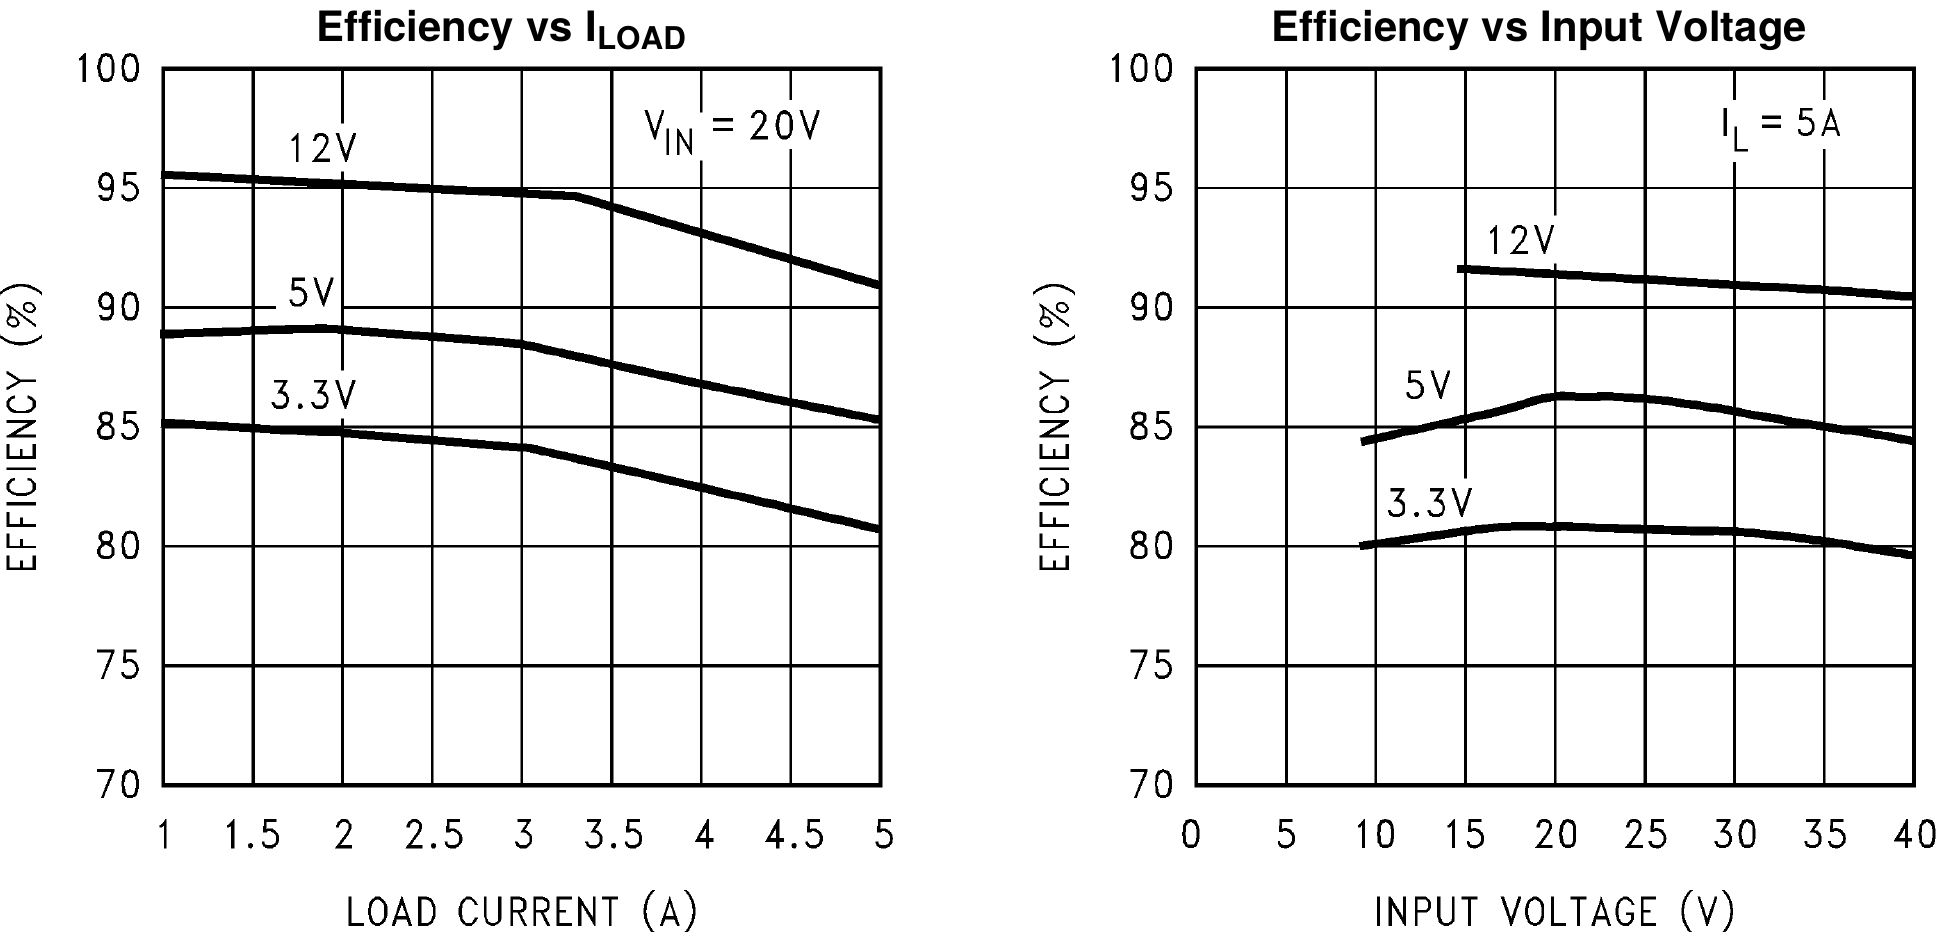
\includegraphics[width=.8\textwidth]{vreg.png}\\
\caption{Regulator Wirkungsgrad}%
\label{fig:vreg}
\end{figure}
Ausgehend von ca. 24 Watt Leistungsaufnahme ($4,8A*5V$) und einem minimalen Wirkungsgrad von 80\%  ergibt sich damit eine überschauliche Verlustleistung von 6 Watt.




\section{Software}

Die Software besteht im Grunde aus zwei Teilen, zum einem der Firmware auf dem \textmu Controller zum anderem aus der Software auf dem NUC, welche die Daten vom \textmu Controller ausließt und über ROS publisht.
In den Folgenden Abschnitten werden Erst die Beiden Softwareteile erläutert, dann wird das Übertragungsprotokoll veranschaulicht.


\subsection{Software auf dem \textmu Controller}
Die Software auf dem \textmu Controller ist vollständig in C++ geschrieben. Eine volständige Dokumentation der Software ist als Doxygen Dokument verfügbar.


\subsection{Client Programm auf der Recheneinheit}
Das Client Programm im folgenden SerialNode genannt 
Im erten Schritt wurde hier ein Python Programm genutzt, welches jedoch einen Nachteil mit sich bringt. Da das ansprechen der seriellen Schnitstelle unter pyserial sehr hohe CPU-Last mit sich bringt.
Da die so verschwendete Rechenleistung für andere Aufgaben benötigt wird und auch energieeffizienz ein wichtiges Kriterium ist, Wurde das Programm erneut in C++ implementiert. Unter verwendung der Systemaufrufe von 
Poll konnte das abfragen der seriellen Schnitstelle auf Systemebene ausgeführt werden, was die effizeinz stark verbessert. Während die Python Implementierung einen CPU-Kern zu 100\%
auslastete liegt die C++ Implementierung im unteren einstelligen Bereich.


\subsection{Übertragungsprotokoll}
Da die Übertragung der Daten via ROS-Serial im ersten Prototypen zu vielen Problemen geführt hat, wurde ien neues Übertragungsprotokoll entwickelt.
Dabei wurde auf Fehlertolleranz niedrigen Ressourcenverbrauch geachtet. Der Datendurchsatz muss hier ausreichend sein um alle Daten stabil mit 100Hz
übertragen zu können.


Der Grundlegende Ablauf der Datenübertragung ist in den Abbildungen [\ref{fig:uC_read}] und [\ref{fig:uC_write}] zu sehen.



\begin{figure}[ht]
\centering
\includegraphics[page=1,width=.8\textwidth]{graph/read.pdf} 
\caption{Lese Daten}
\label{fig:uC_read}
\end{figure}


\begin{figure}[ht]
\centering
\includegraphics[page=1,width=.8\textwidth]{graph/write.pdf} 
\caption{Schreibe Daten}
\label{fig:uC_write}
\end{figure}





